%!TEX root = ../thesis.tex
%*******************************************************************************
%****************************** Second Chapter *********************************
%*******************************************************************************

\chapter{Related Work}

\ifpdf
    \graphicspath{{Chapter3/Figs/Raster/}{Chapter3/Figs/PDF/}{Chapter3/Figs/}}
\else
    \graphicspath{{Chapter3/Figs/Vector/}{Chapter3/Figs/}}
\fi

\section{Introduction}

This chapter discusses background and methods related to 3D shape and pose estimation for articulated subjects. We begin with techniques for correspondence prediction -- a classical method which discusses work focussing on 3D shape and pose estimation for animals. 3D shape and pose estimation for articulated subjects -- primarily animals and humans. We initially focus on skeletal prediction techniques, which output either sets 2D or 3D keypoints. Such techniques are of value to our objective of 3D surface reconstruction, as have been employed in multi-stage pipelines where keypoints are predicted first before a subsequent model fitting stage. The chapter continues with an evaluation of so-called `model-free' techniques, which operate without an explicit template prior.

% Skeletal prediction methods

% Is it a multi-stage approach?
% Does it have a prior?
% 

% Kinect Paper | 

% \section{Point correspondences}
% \section{3D Deformable Model of People and Animals}
% \section{Methods for Single-view Reconstruction}


\section{Predicting point correspondences}

Before delving into methods for 3D reconstruction, it is first necessary to discuss techniques for identifying \emph{point correspondences}. Point correspondences have a long history in computer vision for associating the same real-world location as it is represented by multiple camera views or on a 3D model surface. In a multi-image scenario, determining reliable correspondences between image pairs can be used to greatly reduce the ambiguity when reconstructing 3D scenes from 2D images. Even with only a single image available, correspondences can be predicted between the image and a representative 3D template mesh. This 3D-to-2D correspondence type is important for constraining the class of model fitting algorithms (discussed in depth later) which operate by aligning a 3D template mesh to a given 2D image. Of course, determining point correspondences is made more difficult in the presence of particular nuisance factors. In the case of animal imagery, we must associate points on a non-rigid object with independently moving parts (articulated), deal with frequent self-occlusion in which limbs overlap each other from the perspective of the camera, occlusion caused by environmental factors (e.g. trees, fences, humans etc.), varied and unknown backgrounds and a range of complex lighting conditions (including shadows). Throughout this section, the methods highlighted will be appraised against their suitability in this complex setting.

% https://link.springer.com/article/10.1007/s13735-019-00183-w
% https://arxiv.org/pdf/1603.09114.pdf

\subsection{Relating separate views of the same object/scene}

The first class of techniques focuses on classical approaches for determining corresponding image points taken of precisely the same (and almost always rigid) object. Early techniques focused on stereo~\cite{corres-stereo} or optical flow~\cite{corres-optflow} imagery, and matched image points based on finding regions with similar pixel intensities. Due to the adverse effects caused by changeable environmental factors (e.g. lighting) would have on the appearance of the real-world location when captured in separate images, attention moved towards designing schemes with improved robustness. Improvements were achieved when matching points based on local \emph{mid-level features} such as edges and corners, which have greater invariance to colour changes caused by lighting effects. Typical pipeliens would first identify \emph{interest points} (typically corners~\cite{corner-moravec,corner-harris,corner-susan} or blobs~\cite{sift}), from which local image patches could be compared according to either Squared Sum of Intensity Differences (SSD) or a cross-correlation (CC) scheme. Steady improvements were then made through the design of ever-improving feature descriptors, which encode local image information around points and aim for invariance against common transformations (e.g. viewpoint, rotation and scaling). Progress in this field arguably reached maturity with the advent of SIFT~\cite{sift}, which encodes points according to local histograms of graident orientations and was later speed-up by SURF~\cite{surf} and DAISY~\cite{daisy}. There have been modern attempts to learn sophisticated feature representations using convolutional neural network architectures~\cite{lift, matchnet}, which are shown to offer still further improvement.

The primary aim of these systems is to derive point correspondences between multiple views of the same object, usually as depicted in stereo images or between successive frames of a video. Unfortunately, by matching points based on local geometric features learnt from few image examples, these techniques do not readily extend to identifying correspondences between different instances of the same category. For example, matching SIFT features is likely to result in poor quality correspondences if tested on two dogs of different breeds due to the differing appearance and body geometry. For similar reasons, this class of techniques tend to deteriorate when tested on articulated objects since the object's structure can change and cause self-occlusion between views. The techniques are also known to suffer in scenarios with significant viewpoint changes (e.g. image of the front/back of an animal), since there are few correpsonding points available for matching. Finally, these techniques do not directly offer a method for identifying correspondences between an image and a representative 3D mesh. Although some work exists that extends some of the aforementioned feature descriptors (e.g. 3D-SIFT~\cite{sift-3d}) to 3D, matching typically requires a photorealistic 3D scan of the 2D subject which we cannot assume as input for our problem.

\subsection{Predicting keypoints with a semantic meaning}

This section will explore an alternative class of methods for identifying point correspondences. So far, the approaches described do not detect correspondences with any semantic meaning; in other words, the returned points cannot truly be `named' and there is no guarantee the same points (or even the same number of points) will be identified in different test images. Instead, this section will focus on techniques which predict a set of keypoint locations which are specified in a pre-defined list (for example: nose, tail tip, toe). In general, data-driven machine learning algorithms are used in order to learn an association between image appearance information and semantic keypoint labels. The techniques fall into two general categories: the former set of \emph{supervised techniques} rely on large image datasets manually annotated with keypoint locations, and the latter set of \emph{unsupervised techniques} learn the association through other means. 

\subsubsection{Supervised techniques}

Early work in the supervised prediction of landmarks began through the refinement of object detection methods to predict fine-grained object part labels and eventually progressed to keypoint locations. Perhaps the earliest techniques in this category made use of face part annotations (referred to as fiducial points) to align target faces to improve the face recongition accuracy. Human detection and pose estimation methods progressed from simple bounding box representations~\cite{hog}, to object part prediction~\cite{xxx,xxx}, poselets~\cite{pose-kposelets} and subsequently 2D keypoint localization~\cite{xxx,xxx}. Most commonly, methods aim to predict the location of important 2D human joints (such as the shoulders and wrists) in order to roughly approximate the subject's skeletal pose. For this reason, this task is commonly referred to as \emph{2D human pose estimation}. The earliest techniques represented humans as a graph of parts~\cite{human-rep-parts} and fit shape primitives (e.g. cylinders~\cite{pose-hogg}) to detected edges. Tree-based graphical models known as pictorial structures~\cite{pictorial-structures} were adopted and later made efficient~\cite{pose-felzen}. Improvements were made with models capable of expressing complex relationships betwen joints, such as flexible part mixtures~\cite{yang2013articulated,pose-johnson-mixtureparts}.

Before the popularization of modern deep learning architectures, various methods made use of features computed underneath predicted 2D landmark locations for fine-grained image classification tasks. For this reason, there are limited examples of keypoint datasets for animal categories such as dogs~\cite{liu2012dog} and birds~\cite{WelinderEtal2010}. Chapter 4 of this thesis will discuss StanfordExtra, a new dataset complete with annotated keypoint locations and segmentation masks for 12,000 dog images, encompassing 120 different breeds. At the time of publication, StanfordExtra is the largest annotated animal dataset of its kind. 

% https://arxiv.org/pdf/2012.13392.pdf
Recent works in 2D pose estimation typically employ convolutional neural networks (CNNs) due to the complex feature represenations that can be learnt for joints that, when applied discriminatively, enable accurate recongition. An early example~\cite{pose-embedding} learnt a pose embedding space with a CNN, and employed a nearest neighbour search algorithm to regress a pose. Later, deeper CNN models were used to regress facial point~\cite{pose-face-earlycnn} and full body~\cite{toshev2014deeppose} landmarks. More recent works improve robustness by regressing keypoint confidence maps~\cite{joint-training} rather than 2D keypoints directly, enabling spatial priors to be applied to remove outliers~\cite{cao2018openpose,Pfister15,Pfister14a,Charles16,joint-training,viewpoints-keypoints,pishchulin2016deepcut}. More recent methods are able to directly produce accurate confidence maps through a multi-stage pipeline~\cite{wei2016cpm}. Of particular note are hourglass~\cite{newell2016stacked} (relied upon in this thesis Chapter 3) and multi-level~\cite{sun2019deep,Xiao_2018_ECCV} structures, which combine global reasoning of full-body attributes and of fine-grained details. A related class of methods~\cite{guler2018densepose, taylor2012vitruvian} focus on \emph{dense} human pose estimation, which relate all 2D image pixels to a representative 3D surface of the human body. 

Modern techniques in 2D human pose estimation demonstrate impressive accuracy on in-the-wild datasets, and deal with with parsing multiple subjects in challenging poses and in the presence of various occluders. However, part of what enables these achievements is the prevalance of large 2D keypoint datasets which can be used for training. Further discussion of available 2D keypoint datasets has been left for Chapter 5, in which they are considered in-depth. Further discussion on the history and advances in 2D human pose estimation are comprehensively reviewed in~\cite{2dpose-survey-1, 2dpose-survey-2}.

\subsubsection{Unsupervised learning}

As this thesis focuses on developing methods for animal reconstruction, it is useful to review techniques which operate without large 2D keypoint training datasets, which are scarce for animal subjects. Note that the methods in this section all describe approaches for determining point correspondences between different scenes. Under consideration are methods based on transfer learning, unsupervised learning and methods based on weak-supervision. 

Early correspondence techniques include dense alignment methods including SIFT-flow~\cite{siftflow} which employed optical flow methods to match image using SIFT features, and Bristow et al.~\cite{Bristow2015DenseSC} who demonstrate a method for learning per-pixel semantic correspondences using geometric priors. They also show examples on various animal categories. Recent unsupervised techniques learn \emph{category-specific} semantic priors by employing deep networks on large image collections.

Zhou et al.~\cite{flowweb-efros} demonstrate a method for solving correspondences across an image collection by enforcing cycle consistency. Kanazawa et al.~\cite{kanazawa2016warpnet} introduce WarpNet which predicts a dense 2D deformation field for bird images by learning from synthetic thin-plate spline warps generated on extracted silhouettes. Thewlis et al.~\cite{thewlis-unsup-sphere} apply a similar trick, by ensuring a consistent mapping of warped facial images to a spherical coordinate frame and show results on human and cats. Jakab et al.~\cite{unsup-articulated-objects} show they can estimate 2D human pose without training data data by leverging that between two frames of a simple video sequence, human body shape and texture remains reasonably similar but the pose (including global rotation) varies. They therefore construct an architecture that, given a pair of frames $(I, J)$ defines a network $f$ that given frame $I$ predicts a 2D location vector $y$. The system then combines this vector $y$ with the second frame $J$ and trains a secondary network $g$ to reconstruct the original frame $I$. Due to the limited capacity of $v$, the fact that apart from the pose, most of the information necessary for reconstruction is already available in $J$, the network eventually learns to encode 2D pose coordinates using $v$.

Transfer learning describes a family of methods in which a machine learning model is first \emph{pre-trained} to solve a related task (often making use of secondary dataset with may be larger in size) in order to accumulate knowledge which offers an advantage when solving the original task. DeepLabCut~\cite{mathis2018deeplabcut}, LEAP~\cite{leap-animal-pose} and DeepPoseKit~\cite{graving2019deepposekit} exemplify such techniques, in which existing architectures~\cite{pishchulin2016deepcut,newell2016stacked,densenet,mobilenetv2} are first trained to predict 2D human pose (making use of the large available datasets), and are then repurposed to predict 2D animal keypoints using few (generally 100s) training examples. Cao et al~\cite{animalpose} demonstrate a cross-domain adaptation technique, which transfers knowledge gained from a modestly-sized animal dataset to unseen animal types. There are also dense estimation techniques, which extend DensePose~\cite{guler2018densepose} described above to proximal animal classes~\cite{DenseposeEvo20}, such as chimpanzees, by aligning the geometry between the animal category to humans for which data is plentiful.

% Also under consideration are methods which learn from yet lesser sources of supervision. 

%https://www.robots.ox.ac.uk/~vedaldi/assets/pubs/jakab18unsupervised.pdf
%https://people.csail.mit.edu/celiu/SIFTflow/SIFTflow.pdf
%https://people.eecs.berkeley.edu/~tinghuiz/papers/cvpr15_flow.pdf
%https://www.robots.ox.ac.uk/~vedaldi/assets/pubs/thewlis18modelling.pdf
%https://www.robots.ox.ac.uk/~vedaldi/assets/pubs/thewlis17dense.pdf
%https://www.robots.ox.ac.uk/~vedaldi/assets/pubs/thewlis16fully-trainable.pdf

% https://reader.elsevier.com/reader/sd/pii/S0959438819301151?token=7A13D081FA0EE09BD23EDE5D517D499C7678CD59082C5B225CE01EC8063089BDC30D740FA31FFA6330F7FF6D2FEF2D89
% DeepLabCut: ResNet
% https://www.nature.com/articles/s41592-018-0234-5 (LEAP, StackedHourglass, recently sped up with MobileNet2)
% https://github.com/jgraving/DeepPoseKit
% https://elifesciences.org/articles/47994

% 3D DeepLabCut: https://www.nature.com/articles/s41596-019-0176-0
% AniPose: https://anipose.readthedocs.io/en/latest/
% DeepFly3D: https://elifesciences.org/articles/48571


% TODO: Find out a bit more about sun2019deep, Xiao 2018 etc.

\section{Image segmentation and object detection}

This section will briefly discuss techniques for extracting binary segmentation masks and object bounding boxes for subjects present in input images.


\section{Modelling articulated subjects}

\subsection{Mesh-deformation techniques}

\subsection{Building 3D morphable models}

\subsection{Modelling faces and hands}

\subsection{Modelling humans}

\subsection{Modelling animals}

\section{Model-based methods for non-rigid reconstruction}

\subsection{Model-based faces and hands}

\subsection{Model-based human pose estimation}

\subsection{Model-based human shape and pose}

\subsection{Model-based animals}

\section{Model-free methods for non-rigid reconstruction}

\subsection{Shape-from-X}





large dataset on large large Techniques in this section typically achieve this using data-driven machine learning algorithms, which can be trained on various  general, data-driven machine learning algorithms are used to predict an association between image pixels and locations with a semantic meaning. techniques used to achieve this techniques achieve this In general, data driven machine learning techniques are used to train an algorithm to associate image appearance features with semantically-meaningful partsIn order to teach a system to understand semantic this section, we will discuss techniques for predicting keypoints from a pre-defined list

These approaches do offer some advantages; in particular, the approaches do not require a training procedure based on a labelled dataset, although the techniques cannot be used to associate image points to a representative 3D mesh. In this section, we will discuss techniques for predicting points from a pre-defined list 

a labelled dataset this does offer some advantages (particularly that the approaches do not require a labelled dataset for training, data 

and in general, the number of correspondences the number of detected correspondences can differ between test examples and there is no pre-determined there is no pre-determined list of detected correspondences points the methods should obtain, and in general the number of returned keypoints can differ  used for identifying 2D image points based on a pre-defined   approach to identifying image points, although this time the desired locations will are pre-defined.

\begin{enumerate}
    \item Talk about all 2D keypoint detection techniques
    \item Talk about 
\end{enumerate}



For example, For example, techniques such as SIFT generate different feature descriptions for two points taken on different zebras, due to the different patterns. Such systems also struggle greatly under object-viewpoint, particularly for 

which relies on local gradient information will generate different feature descriptions for two points taken on different zebra since the patterns may differ. The next class of techniques are designed to overcome this limitation, and offer matching based on \emph{semantic point correspondences}.




% unfortunately, these techniques 

% such as to ensure uniqueness ensure specificity and comparing feature descriptors computed from them. Early feature descriptors focus only Feature descriptors often capture local statistics related to the image location and aim to have some invariance to different lighting conditions, scales, rotations or other transforms. from which  (typically repeatible features such as edges Techniques fall into two categories: global image descriptors are calculated on the whole image, and have some advantages in that they are invariant to matching based on the whole image, and have some advantages since they are naturall invariant to invarient 

% majority of techniques solve matching based on local image-features, techniques match based on local features, i.e. rely on general, techniques are used to identify so-called \emph{interest points} which have some repeatibility properties for which a \emph{feature descriptor} can be Historically, the most successful methods operate by Early techniques designed for stereo matching and for optical flow were designed to operate under small viewpoint changes, but early technique proved suitable for stereo matching under small viewpoint changes, but was not rotation invariant and for deriving point correspondences since the 1980s, echniques for deriving point correspondences between images has existed since the 1980soperated on image pixel intensity values, without much consideration for the underlying objects. Improvements were made with geometric techniques, such as edge and corner detectors, which offered some robustness to varying lighting conditions. However, the mid-level features represenations of SIFT~\cite{}, HOG~\cite{}, DAISY~\cite{}, VLAD~\cite{} etc. offered considerable improvements, allowing point matching under various object scales and camera viewpoints.

% However, while suitable for processing such techniques were unfortunately unable to match semantically-meaningful keypoint locations across different object instances

% the feature representations of techniques struggle with varying camera viewpoints, still typically fail when 

% at some robustness to that related mid-level appearance features, such as corners 

% Major imawithout consideration for the objects they purely on image pixels, with little knowledge of the objects they Of course, determine which 2D image locations are in correspondence 

% The history of deriving point correspondences begins with stereo and optical flow, which use 

% Even the earliest reconstruction techniques, such as in stereo or optical flow based methods, rely on point correspondences to determine 3D structure. 

% to use of point correspondences to 


% For example, imagine we have captured multiple images ${I_1, I_2, ...}$ of the same static scene containing a dog. A classical approach for recovering the 3D 3D dog For example, imagine we have various images captured of the same static scene containing a dog. In order to determine the consider a real-world point on the end of a dog's nose for which we have yet to determine the true 3D world location. To recover the 3D point, we may start by grouping together projections of this point $\{(u_i, v_i)\} \in R^2$ in various images we have captured of the scene. From these point correspondences, we could begin 


% we may start We may start by grouping together various projections of this point in various images we have captured of the scene From various images captured of the scene, we may start by grouping together the various projections of this nose point it is useful to group together the various projections of this point . Further, we can various projections of this point in on the end of a dogs nose, scene containing a dog, we can group to group 2D image points 

% points a scene containing a dog, we may wish to group , whether in related locations between two images, an image and a 3D surface or two 3D surfaces. Often, point correspondences are used to group together multiple image views of the same real-world location, or to relate an image point with a location on a representative 3D surface. 


% Throughout the long history of 3D reconstruction, nearly all methods which focus on recovering complex 3D objects from 2D image data make use of \emph{point correspondences} to constrain the problem. By understanding which pairs of Early work focuses on \emph{image matching} to 


% In order to reconstruct a complex 3D object from 2D image data, we typically require significant constraints from Techniques which reconstruct complex 3D subjects from 2D image data typically require 

% In order to reconstruct a complex 3D subject from 2D image data, it is almost always essential to constrain  3D articulated subject from 2D image data, it is almost always image, it is alms3D reconstruction has a long history 3D reconstruction techniques have a long history in reconstruction, and nearly all require as 

\begin{enumerate}
    \item 3D reconstruction techniques rely upon point correspondences. This has a very long history:
    \item Optical flow, mid-level discriptors (SIFT, DAISY etc.)
    \item More recently, pose estimation techniques have found themselves useful 
\end{enumerate}




\section{Modelling articulated subjects}

\section{Skeletal prediction}

The first class of techniques, known as \textit{skeletal prediction} methods, output sets of either 2D or 3D keypoint locations. Since only a skeleton outline is obtained, apart from basic limb measurements, no other shape detail (e.g. surface definition, object density etc.) is obtained. However, it should be noted that this output form is often perfectly satisfactory depending on the intended application. In particular, this family of techniques have found numerous applications in controllerless gaming (e.g. Microsoft Kinect~\cite{kinectpaper}), motion capture (e.g. for digital character generation~\cite{xxx}), gait analysis (e.g. identifying lameness in cattle~\cite{xxx}) and many more. 

Early approaches in this category build statistical models of limb lengths and poses using freely available motion capture data~\cite{barron2001estimating}. These are then used to adapt a digital skeleton to fit each frame of an input video sequence.  

    \subsection{Kinect skeletal tracking}
    Shotton et al.~\cite{kinectpaper} designed a human skeletal tracking capability, which was later incorporated into the Microsoft Kinect Sensor SDK (see Figure \ref{fig:kinect_skeleton}. A large motion capture database containing approximately 500K frames was captured from human subjects performing a wide variety of activities (e.g.\ driving, dancing, kicking, running, etc.). This dataset was then used to drive a generative body model (constituting strong prior knowledge for this problem) which could be sampled from to create synthetic depth images with dense body part labels. A random forest classifier is then used to predict these body labels on unseen examples. A per-pixel density estimator for each body part is calculated for each 3D world space coordinate based on: (1) the inferred body part probability for the projected pixel, (2) the world surface area of the pixel. Density estimators for each body part are then used in combination to localize particular body joints, which are annotated with a calculated confidence value. 

    \begin{figure}[H] % Example image
        \center{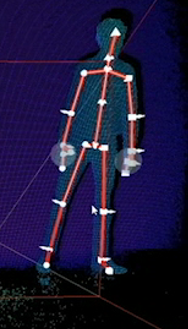
\includegraphics[width=0.25\linewidth]{human_tracking}}
        \caption{Kinect generating per-pixel joint proposals.}
        \label{fig:kinect_skeleton}
    \end{figure}

    \subsection{Multi-stage approaches}
    More recent approaches are either predict 2D joint positions on an input image, and use a subsequent step that `lifts' these to a 3D pose, or predicts the 3D pose directly. Note that both approaches must overcome significant ambiguity. Determining joint positions is a task made challenging due to large variations in visual appearence, commonly due to clothing, body shape and camera view. As explained by Toshev and Szegedy~\cite{toshev2014deeppose}, even with perfect joint locations the subsequent lifting step is also ill-posed, as the space of consistent 3D poses for given 2D landmark locations is infinite. This is typically resolved using strong prior knowledge which usually takes the form of 3D geometric pose priors and temporal or structural constraints. Examples of such systems include DeepPose~\cite{toshev2014deeppose}, an approach which employs a CNN to reason jointly about 2D landmark detection and 3D pose estimation from single RGB images. Pishchulin et al.~\cite{pishchulin2016deepcut} later introduced DeepCut which extends DeepPose to the multi-person case. Both systems are trained on large body joint databases. 

    \subsection{Direct approaches}
    However, some direct techniques exist which do not require an initial 2D joint prediction. These include methods that directly regress to a 3D pose~\cite{tekin2016direct}. However, these typically rely on an annotated set of 3D joint labels, which can be difficult and costly to obtain, or being able to build a representative synthetic dataset, which is non-trivial task.

    %% Discuss Amazon's system, Novotny's system etc.

    \subsection{Applicability to animal categories}
    % 2D predictor DeepLabCut 

\section{Model-free shape and pose estimation}

This section will discuss methods for dense 3D reconstruction. 

\begin{enumerate}
    \item PiFu and Neural Radiance Fields
    \item Novotny dense 3D prediction
\end{enumerate}

\section{Model-based shape and pose estimation}
    Model (or mesh) fitting encompasses a set of methods that work by adapting a 3D template mesh to either an input image or input video sequence. Such techniques therefore return a full 3D model intended to faithfully reconstruct the performance given by the tracking target, although the accuracy of this reconstruction is heavily conditioned on the quality of the method.
    

    \subsection{Form of the template prior}
    A polygon mesh $M = (V, T)$ is a collection of vertices, edges bound by vertex pairs, and polygons bound by sequences of edges and vertices~\cite{smith2006vertex}. Although other convex shapes are allowed, mesh polygons will always be considered triangular (and hence referred to as \emph{triangles}) unless explicitly stated otherwise. An example mesh is shown in Figure~\ref{fig:polygon_mesh}. 
    
    \begin{figure}[H] % Example image
        \center{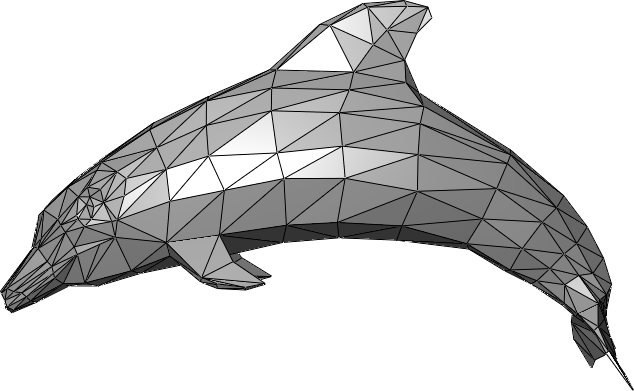
\includegraphics[width=0.5\linewidth]{dolphin_mesh}}
        \caption{A polygon mesh~\cite{polygon_mesh}.}
        \label{fig:polygon_mesh}
    \end{figure}

    
    \subsection{Mesh deformation}
    The process of adapting a 3D mesh is known as \textit{mesh deformation} and is common across many computer graphics applications, particuarly those in which models are designed to represent dynamic objects. To constrain an optimization function (or simplify the animation process), it is useful to introduce priors that prevent unnatural mesh movement. Two methods for achieving this are discussed:

        \subsubsection{Skeletal Rigging and Linear Blend Skinning}
        In cases that the mesh shape is known in advance, it is common to follow a process known as \textit{rigging}, in which the mesh is augmented with a hierarchical bone structure. The point at which two bones meet is called a \emph{joint}, and these can be used to define acceptable centres of rotation for mesh deformation. It is possible to describe a distribution of joint configurations, which could be used to constrain the mesh to (in the case of human / animal subjects) anatomically achievable poses. It is also simple to define conceptual `body parts' from a rigged mesh, by considering regions between pairs of joints; for example a lower leg region can be defined between a knee and ankle joint. A simple example of a rigged 2D mesh with joints indicated by green diamonds is shown in Figure~\ref{fig:finger_model}. Note how the mesh surface deforms naturally as the joints are displaced.
        
        \begin{figure}[H]
            \centering
            \begin{subfigure}{0.48\linewidth}
            \centering
                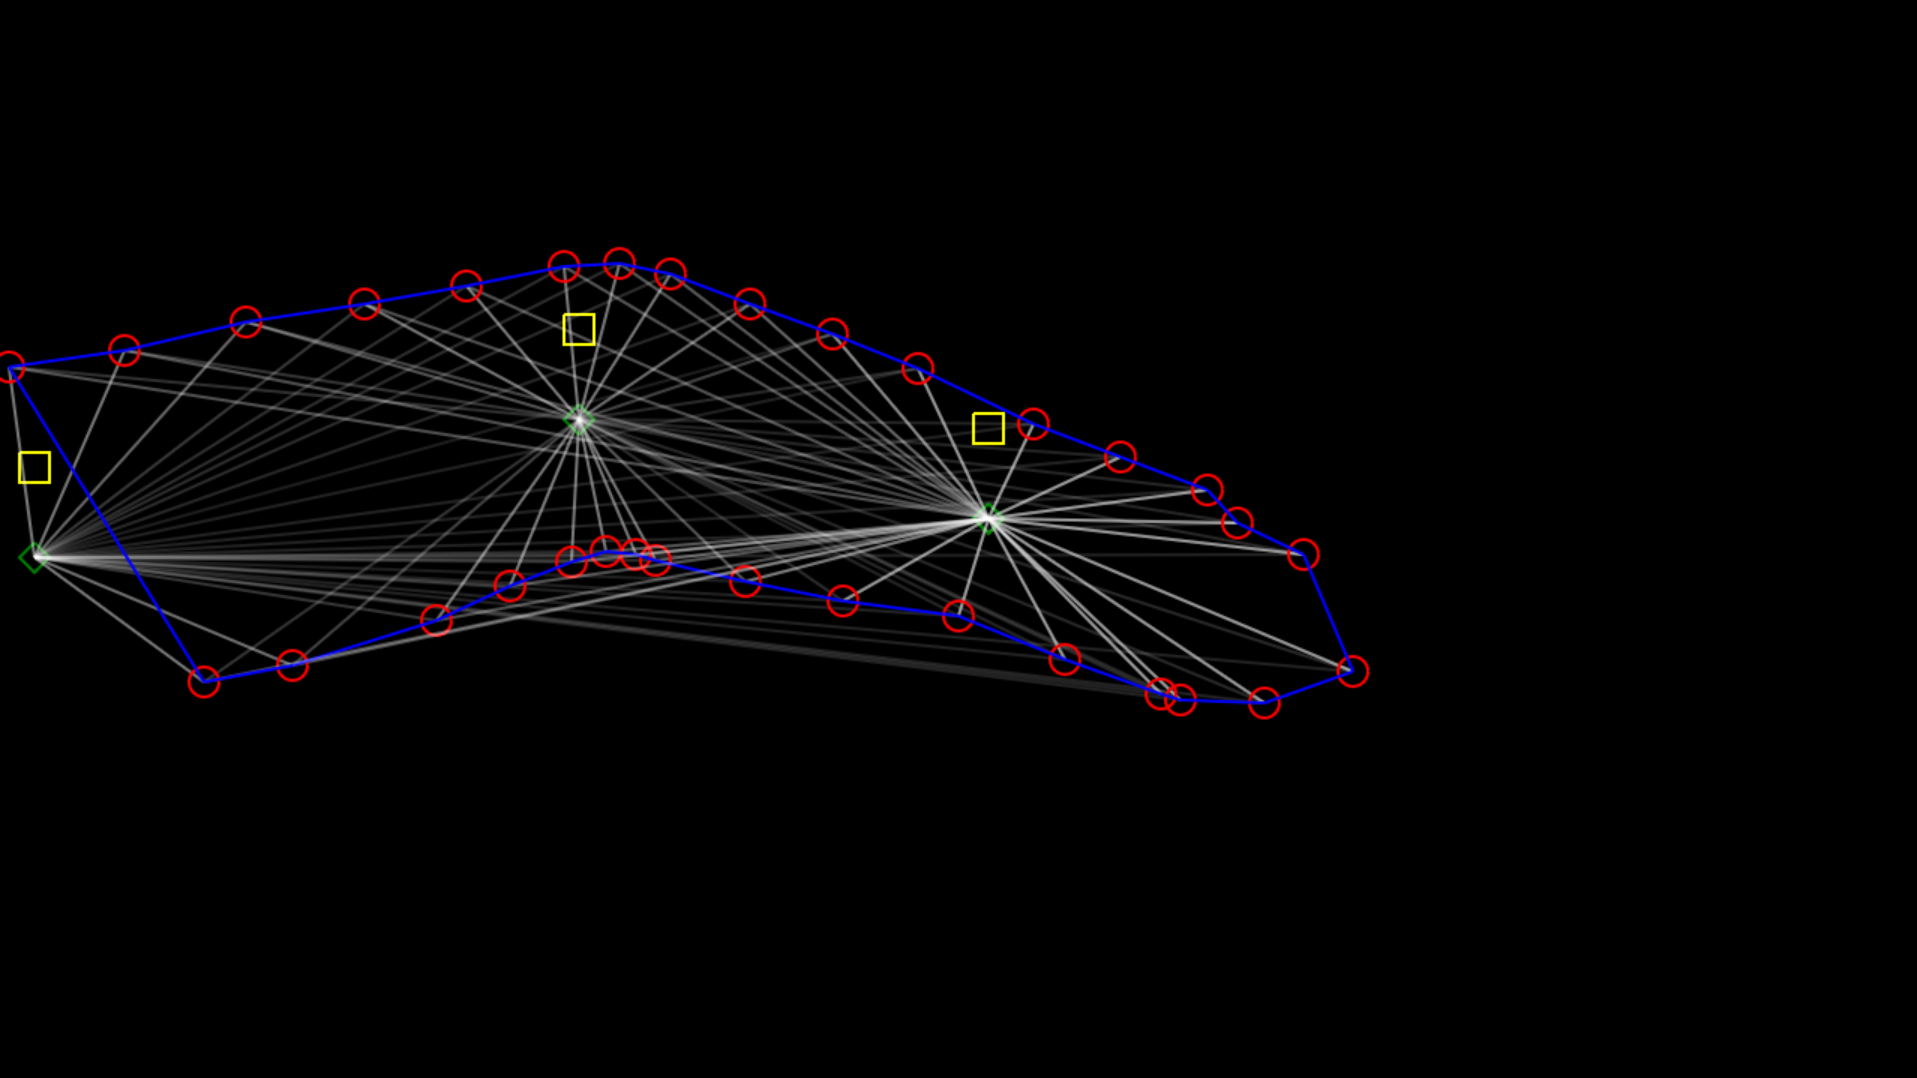
\includegraphics[width=1\linewidth]{finger/finger1}
                \caption{Default joint positions.}
            \end{subfigure}
            \begin{subfigure}{0.48\linewidth}
            \centering
                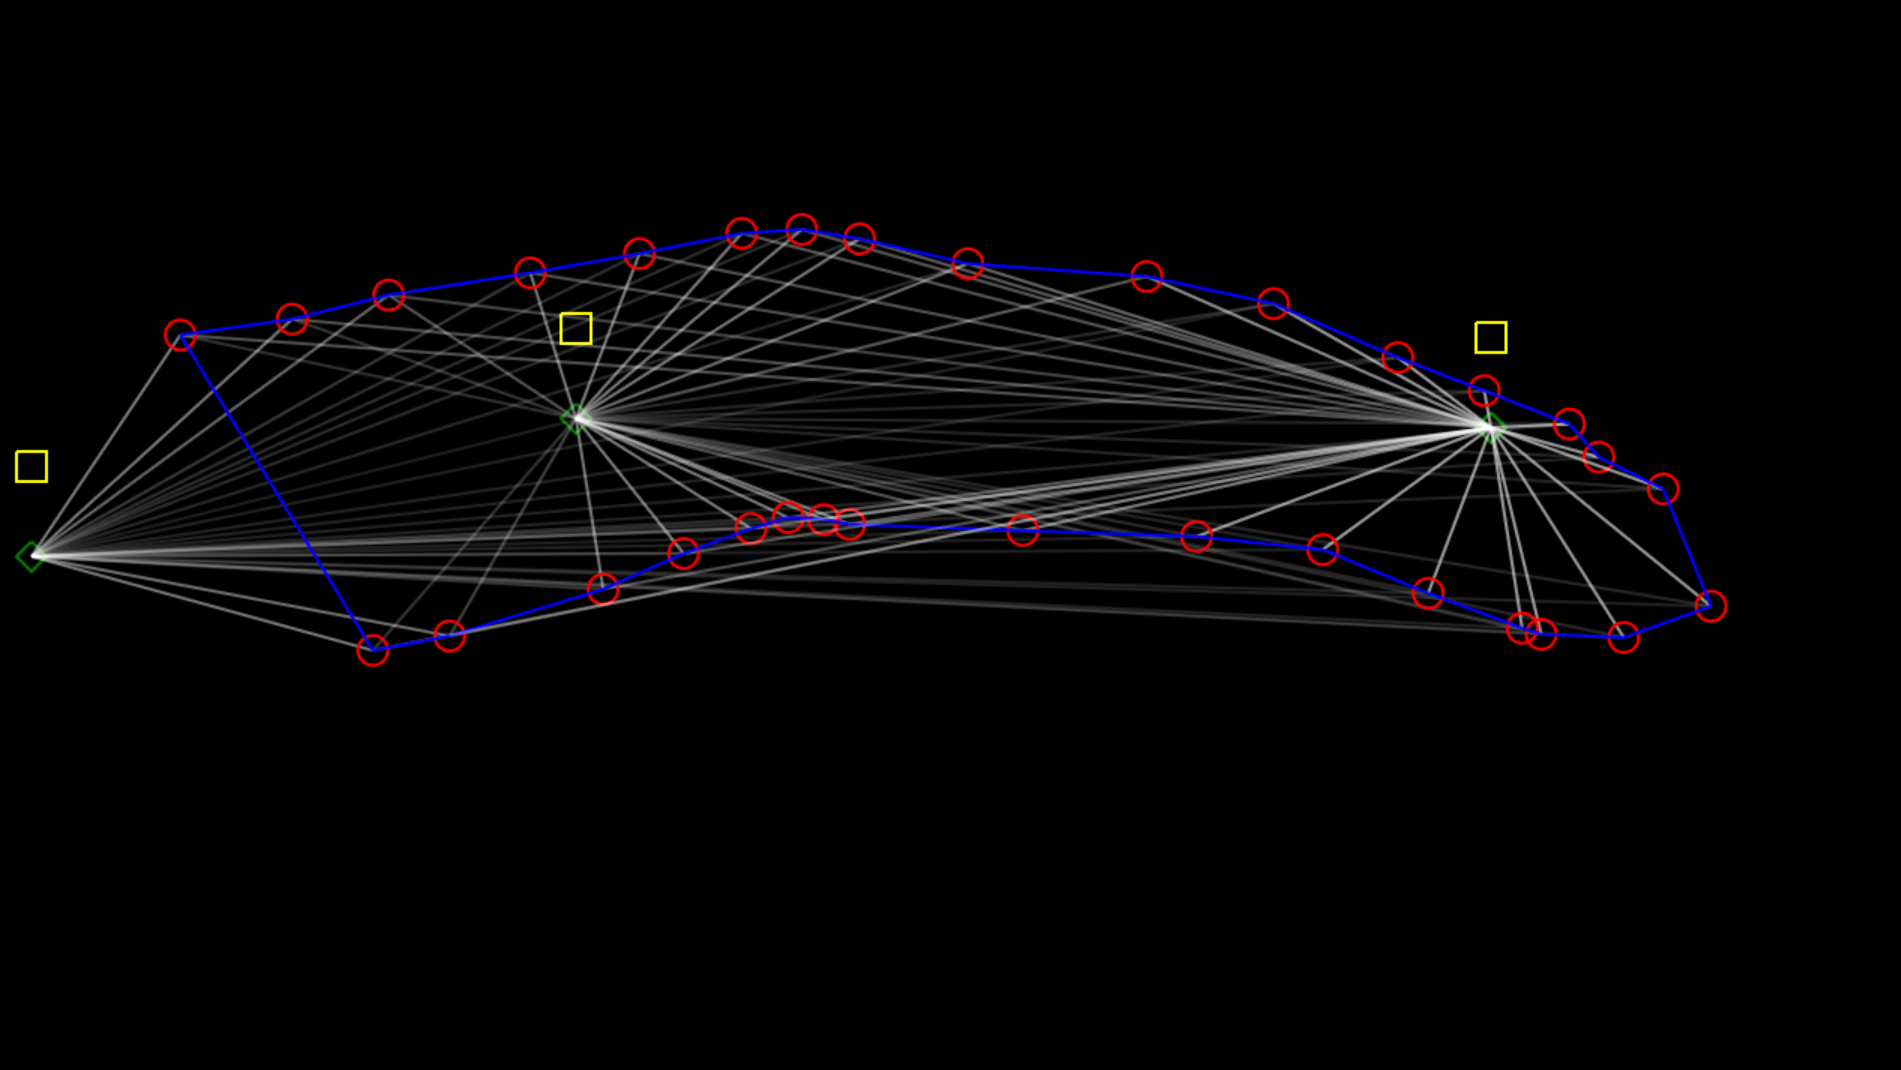
\includegraphics[width=1\linewidth]{finger/finger2}
                \caption{Right-most joint displaced.}
            \end{subfigure}
            \begin{subfigure}{0.48\linewidth}
            \centering
                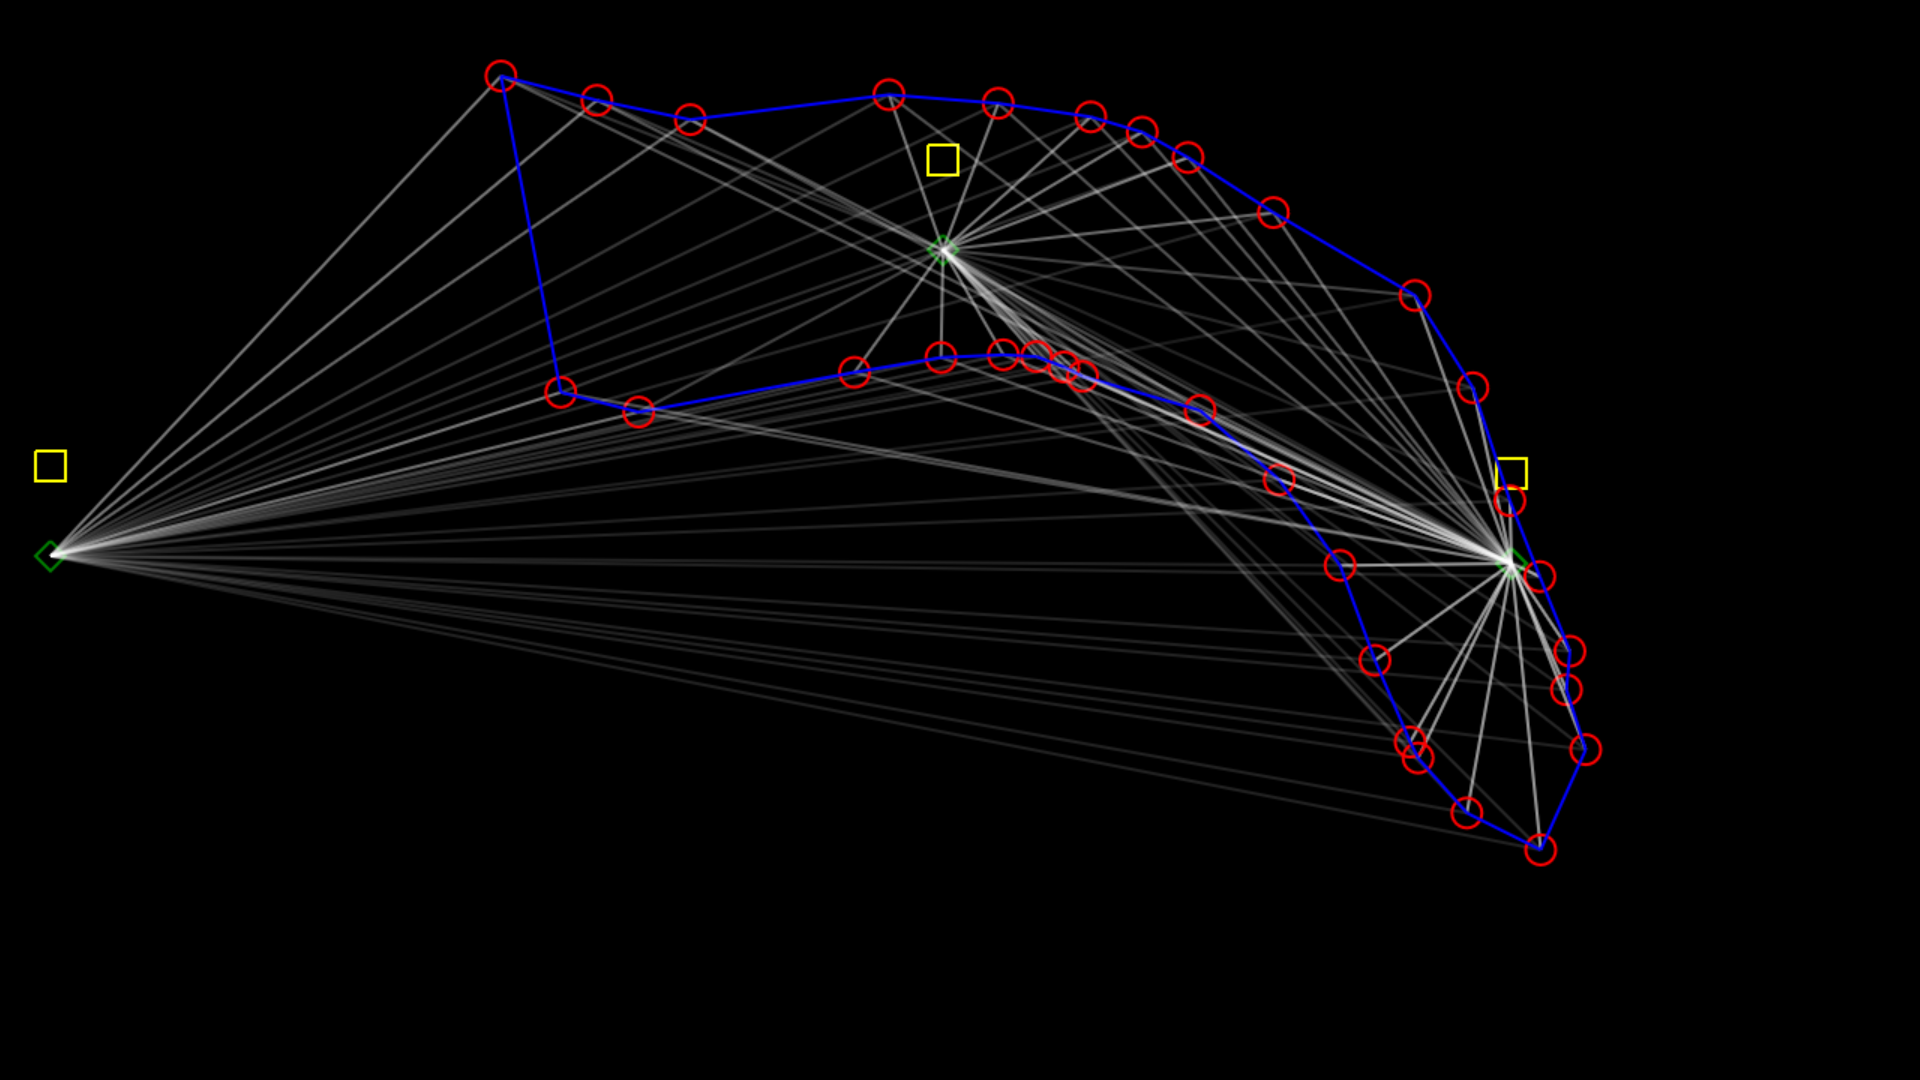
\includegraphics[width=1\linewidth]{finger/finger3}
                \caption{Central joint displaced and right-most joint displaced and rotated.}
            \end{subfigure}%
            \caption{Web application demonstrating LBS on a 2D finger mesh. Joints are denoted as green diamonds.}
            \label{fig:finger_model}
        \end{figure}

        \clearpage
        Formally, a skinned mesh consists of a set of rigged vertices $V \subseteq \mathbb{R}^3 \times \mathbb{R}^{|J|}$, a set of faces $F \subseteq V^3$ and joints $J \subseteq R^{3\times3}$. Each vertex $v = (x, s) \in V$ consists of positional coordinate $x \in \mathbb{R}^{3}$ and a weight vector $s \in \mathbb{R}^{|J|}$ which describes the level of influence each joint $j \in J$ has over its movement. Many approaches exist for assigning weights, but perhaps the simplest is to build a vector with entries corresponding to the distance from the vertex to each joint centre. Skinning weight vectors are normalized such that their entries sum to one, and for computational reasons, the number of non-zero elements is typically limited to 2 or 4. The weakness of such models is that artifacts and other unrealistic deformations can occur around the model joints, particularly for meshes that model non-linear structures such as humans. However, the technique is frequently used in computer graphics and game design when a character's shape is known ahead of time.

        To assist in explanation, Figure \ref{fig:rigged_cylinder} shows skinning weight influences from three joints within a rigged cylinder mesh. Here, $|J| = 3$ and each vertex $v_{i} = (x_{i}, s_{i}) \in V$ has a skinning weight vector $s_{i} \in \mathbb{R}^{3}$. Each model joint is assigned a distinct RGB value, shown separately in (a), (b) and (c), and together in (d) by linearly combining the colours. This linear blend colorization scheme will be frequently used in later sections of this report.

        \begin{figure}[H]
            \centering
            \begin{subfigure}{0.25\linewidth}
            \centering
                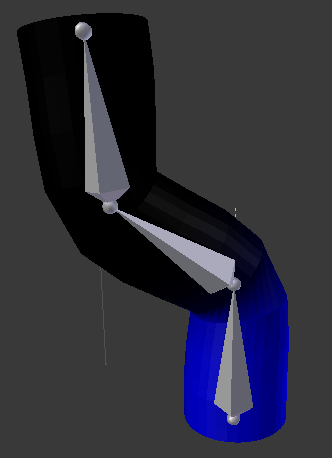
\includegraphics[width=1\linewidth]{wonky_pole/lower_bone}
                \caption{Lower joint.}
            \end{subfigure}%
            \begin{subfigure}{0.25\linewidth}
            \centering
                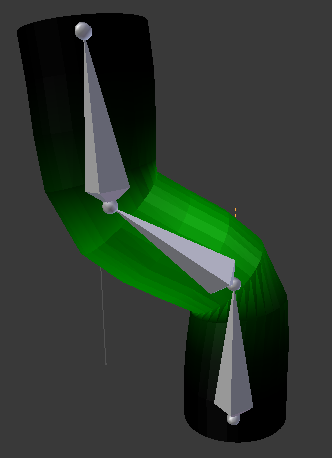
\includegraphics[width=1\linewidth]{wonky_pole/middle_bone}
                \caption{Middle joint.}
            \end{subfigure}%
            \begin{subfigure}{0.25\linewidth}
            \centering
                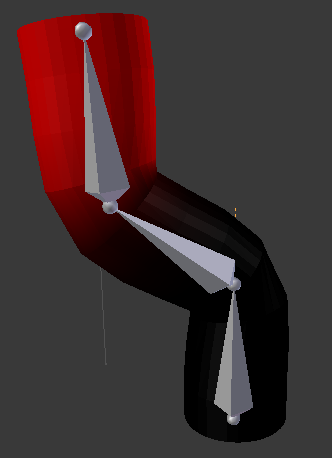
\includegraphics[width=1\linewidth]{wonky_pole/upper_bone}
                \caption{Upper joint.}
            \end{subfigure}%
            \begin{subfigure}{0.25\linewidth}
            \centering
                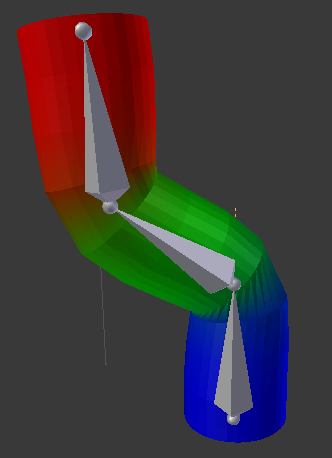
\includegraphics[width=1\linewidth]{wonky_pole/linear_blend}
                \caption{Linear blend.}
            \end{subfigure}%
            \caption{A rigged cylinder with $|J| = 3$ and where each vertex $v_{i} = (x_{i}, s_{i}) \in V$ has a skinning weight vector $s_{i} \in \mathbb{R}^{3}$.}
            \label{fig:rigged_cylinder}
        \end{figure}

        Figure \ref{fig:rigged_quadruped} shows a more complex rigged quadruped mesh with $|J| = 25$ with skinning weight influences again shown by the linear blend colorization scheme. Again, each joint is assigned a unique RGB value and a vertex's colour is calculated by linearly combining joint colours with skinning weight vectors given by the $\{s_{i}\}$. A triangle's colour is then generated by averaging the colours given for the three surrounding vertices.

        \begin{figure}[H] % Example image
            \center{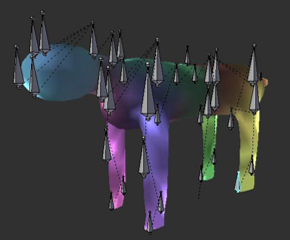
\includegraphics[width=0.5\linewidth]{linear_blend_bold_bones}}
            \caption{A rigged quadruped with $|J| = 25$ and where each vertex $v_{i} = (x_{i}, s_{i}) \in V$ has a skinning weight vector $s_{i} \in \mathbb{R}^{3}$. Visualization uses the linear blend colorization scheme in which each joint is assigned a unique RGB value.}
            \label{fig:rigged_quadruped}
        \end{figure}

        Once a mesh has been suitably rigged, there are a number of options (e.g. Linear Blend Skinning (LBS), Dual Quaternions~\cite{kavan2007skinning} etc.) for applying a particular mesh deformation. Typically, a user assigns a transformation (in this case comprising a rotation and transformation) to each `joint' and the updated positions $\bar{x_{i}}$ of the remaining vertices $v_{i}$ with original positions $x_{i}$ are then calculated. The original transformation for each joint (i.e. before the deformation) is expressed as a matrix $U_{j}$. The transformation after the deformation has been applied is captured by $D_{j}$. Note that $s_{ij}$ denotes the skinning weight influence of joint~$j \in J$ on vertex $v_{i} \in V$.
        
        The updated positions $\bar{x_{i}}$ can then be calculated by LBS:

        \begin{equation}
            \bar{x_{i}} = \sum_{j=1}^{|J|}s_{ij}D_{j}U_{j}^{-1}x_{i}
        \end{equation}

        \clearpage
        \subsubsection{Rendering}
        The process of generating a 2D image from a 3D polygon mesh is known as rendering and can be achieved through a process known as raytracing. Raytracing is a rendering technique able to generate photorealistic 2D images from the scene. It can be considered the opposite process by which the human eye perceives the world, as this method involves lines being cast outwards, beginning at a point known as the \emph{camera origin}. Figure \ref{fig:raycasting} shows a typical set up, in which rays are cast from the camera origin through each pixel on the image plane. The colour for the pixel is obtained by following the ray through the scene until a light source or non-reflective surface is reached, taking into account any reflections or non-opaque scene items. Due to the considerable comptuation required, the operation is often parallelized and assigned to the GPU. However, the technique is typically considered unsuitable for real-time rendering of complex scenes (due to complex ray paths) or when high resolution images (many rays required) are needed. However, for this work, scenes are typically made up of a single non-reflective, solid mesh surface and contain no complex elements (e.g.\ shadows, non-constant lighting.

        \begin{figure}[H] % Example image
            \center{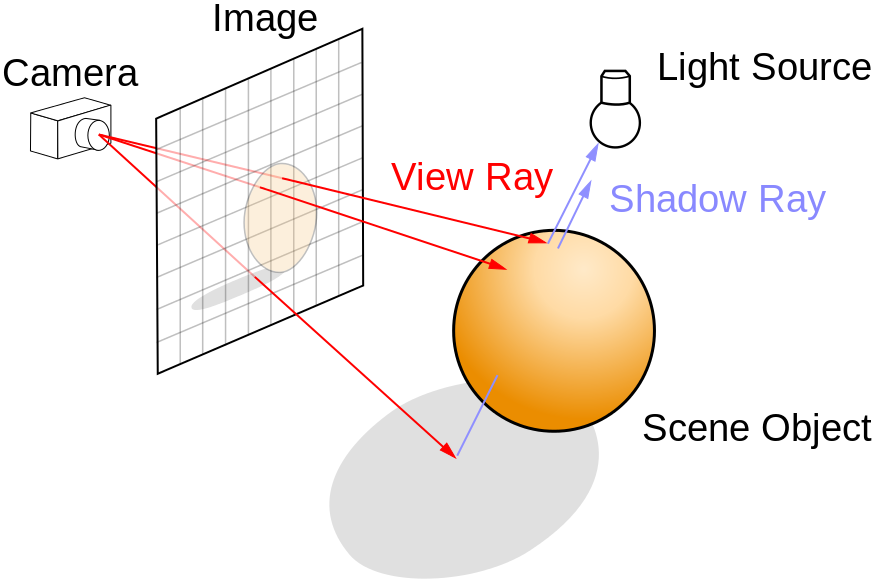
\includegraphics[width=0.5\linewidth]{ray_trace}}
            \caption{Diagram showing raycast rendering.~\cite{rendering}.}
            \label{fig:raycasting}
        \end{figure}

        It is also worth noting that the standard method for raycasting is not differentiable, causing problems for differentiable optimizers (including neural networks). However, alternative rendering methods~\cite{loper2014opendr} are available for these purposes.


    \subsection{Approaches}
    The following section describes an number of existing model fitting methods.

    \subsubsection{Model fitting: fitting a template model to correspondences}
    % Edit to talk about e.g. SMPLify

    %  Model fitting algorithms are typically provided with point correspondences between the template mesh and input images in order to help constrain the optimization. Correspondences are either provided by a human annotator or predicted by a discriminative machine learning model.

    Taylor et al. demonstrate a model fitting approach that operates on a rigged 3D human mesh~\cite{taylor2012vitruvian}. Their aim is to learn a set of pose parameters $\theta \in \mathbb{R}^{d}$ so as to explain a set of image points $D = \{x_{i}\}_{i=0}^{n}$. Data points $x_{i} \in \mathbb{R}^{3}$ are collected from a calibrated depth camera. Once these pose parameters are learnt, the mesh is deformed according to the LBS algorithm defined above.

    The template mesh contains $|J| = 13$ joints, and $m$ skinned vertices ${V} = \{v_{i}\}_{i=1}^{m}$. Again, each vertex $v_{i} \in V$ is defined as:

    \begin{equation}
        v_{i} = (x_{i}, s_{i})
    \end{equation}
    where $x_{i} \in \mathbb{R}^{3}$ represents the base 3D vertex positions in a canonical pose $\theta_{0}$ and the $s_{i} \in \mathbb{R}^{|J|}$ are skinning weight vectors. It is possible to define a mesh induced by a pose $S(\theta) = (V, T)$ for vertices $V$ and triangles $T$. Due to the resemblance of the mesh surface induced by the canonical mesh pose $\theta_{0}$ and Da Vinci's Vitruvian man~\cite{davinci}, this surface is referred to as the \emph{Vitruvian Manifold}, and is shown in Figure~\ref{fig:vitruvian_man}. 

    \begin{figure}[H] % Example image
        \center{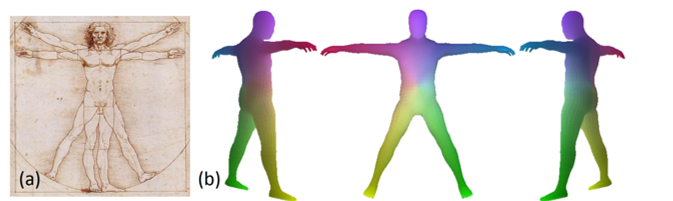
\includegraphics[width=0.95\linewidth]{vitruvian_man}}
        \caption{(a) Vitruvian Man by Leonardo da Vinci~\cite{davinci} and (b) the Vitruvian Manifold reprinted from~\cite{taylor2012vitruvian}.}
        \label{fig:vitruvian_man}
    \end{figure}

    The primary contribution of this paper is the design of a model able to predict \emph{dense correspondences} between the 3D canonical mesh and input 3D images. In other words, \emph{every} body pixel on an input image is regressed to a point on the vitruvian manifold mesh. The authors demonstrate the accuracy of these correspondences is sufficient for \emph{one-shot learning}, meaning there is no need to recalculate correspondences after a subsequent optimization step. The reason for this is the strength of the core error term which penalizes the sum of errors between image points $\{x_{i}\}_{i=0}^{n}$ and determined mesh correspondences $U = \{u_{i}\}_{i=0}^{n} \subseteq V$:

    \begin{equation}
        E_{\text{data}}(\theta,U) =\sum_{i=1}^{n}s_{i} \cdot d(x_{i}, M(u_{i}; \theta))
    \end{equation}
    where $M(u_{i}, \theta)$ is the position of vertex $u_{i}$ on the vitruvian manifold mesh after having been displaced by an LBS deformation with respect to the pose~$\theta$. 

    The sheer quantity of correspondences greatly constrain their optimizer which works well, even on challenging input images. Much of this report focuses on how this paper can be extended to work for animal subjects, incorporating deep learning correspondence prediction and working from monocular RGB input data.

    \subsubsection{Model parameter regression}

    This is how you do this using a deep network. 


We want to do model based reconstruction to impose a prior on the fitting and also automatically recover an interpretable fit. 

\subsection{Fitting to animal video sequences}
Stebbing et al.~\cite{arap_stebbing} introduce a technique capable of fitting a template mesh to live video sequences for a range of different animal species. Some user interaction is required in order to segment the animal from the background and to provide sparse 3D-mesh-to-2D-image key point correspondences. This work only operates on input video sequences (rather than single frames), so a number of temporal terms are incorporated that encourage sensible inter-frame model deviation. The system requires an annotated input template mesh representative of the target animal species. Note that this work does not require the template mesh to have an inner skeletal structure. However, the user assists an ARAP-style term by assigning each mesh vertex $v_i$ to one of $M$ groups which share a set of basis rotations $B_{m}$. 

\begin{figure}[H]
    \centering
    \begin{subfigure}{0.5\textwidth}
    \centering
        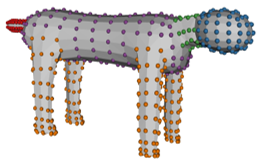
\includegraphics[height=0.5\linewidth]{arapsfm/arap_annotated_template}
        \caption{Template mesh with joint movement constraints.}
    \end{subfigure}%
    \begin{subfigure}{0.5\textwidth}
    \centering
        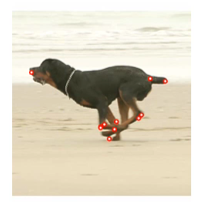
\includegraphics[height=0.5\linewidth]{arapsfm/arap_point_tracks}
        \caption{Example of user supplied point tracks.}
    \end{subfigure}%
    \caption{User input required for the deformable mesh animation algorithm, reprinted from~\cite{arap_stebbing}.}
    \label{fig:arap_user}
\end{figure} 

Through reasonably accurate pose fitting and by allowing some pose-invariant shape deformation, this work produces smooth meshes which are often a good match to the input video. Moreover, their experimentation shows that ARAP is a useful prior for reconstructing articulated, non-rigid motion in instances that an internal skeleton is a priori unknown. However, the shape attributes for the reconstructed model are not particularly accurate, which results in frequent errors appearing at internal occluding contours. In addition, the large non-convex optimization algorithm is an expensive operation, taking around 1 minute per video frame on a standard Linux workstation.

Results showing this work fitting a crude dog template mesh to a sample video obtained from YouTube are shown previously in Figure \ref{fig:intro_arap_output}. Figure \ref{fig:arap_output} shows another example, which operates on a template impala mesh.

\begin{figure}[H]
    \center{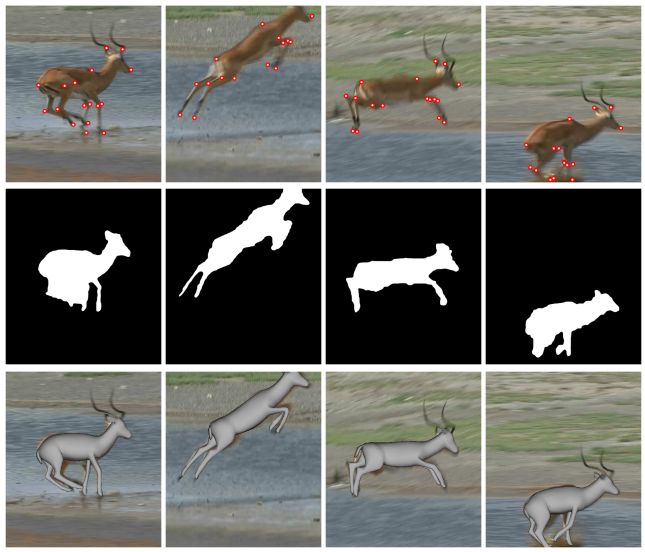
\includegraphics[width=0.95\linewidth]{arapsfm/arap_impala}}
    \caption{Example of an impala template being fit to input video sequence, reprinted from~\cite{arap_stebbing}}
    \label{fig:arap_output}
\end{figure}

\subsection{Learning animal shape from unrelated 2D images}
Cashman and Fitzgibbon~\cite{cashman2013shape} introduce an optimization technique able to recover a parameterized, morphable 3D model from unrelated 2D images depicting examples of the target class. The method requires user-supplied 2D object outlines and point constraints for each image, and a single rigid mesh for the entire object class. The authors demonstrate recovering an 8-parameter morphable dolphin model from 32 images obtained from Google. To reduce required user activity, it is reasonable to assume that given sufficient labelled training data, it would be simple to manipulate a convolutional network architecture able to perform foreground / background segmentation and identify human key points (say, joints) for the desired object class. The system achieves impressive results when optimizing over both pose and shape parameters across a range of object classes, but struggles for articulated models such as polar bears.

\begin{figure}[H] % Example image
    \center{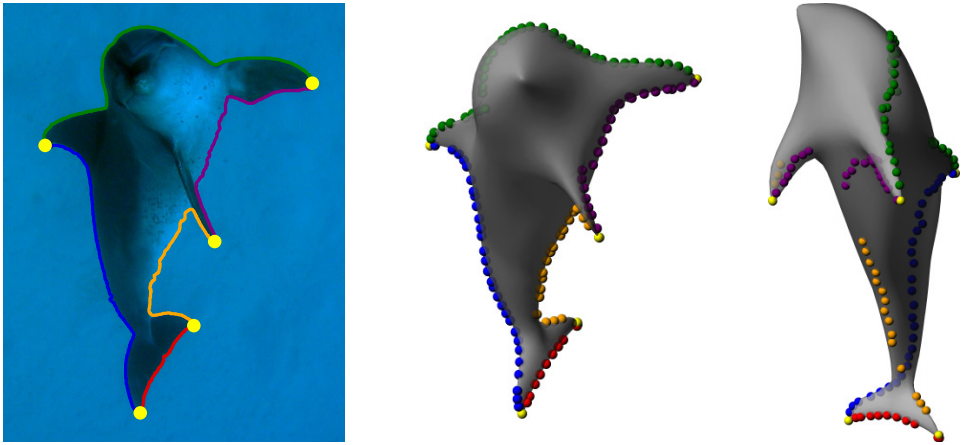
\includegraphics[width=0.7\linewidth]{dolphins}}
    \caption{8-parameter dolphin model with annotated contour (left) and contour generators (middle and right).}
    \label{fig:cashman_fitzgibbon}
\end{figure}

\subsection{Fitting to an articulated hand model}
Given the availability of strong shape and pose priors, articulated hand tracking aptly demonstrates the advantage of model fitting approaches. Again, it is first necessary to decide how the human hand should be parameterized, i.e. what an optimizer should specifically aim to learn. Similar to the case with the full human body, the aim is again to adapt a mesh (although this time of a hand) to reproduce a performance given by a real human hand either in still frames or from an input video sequence. Many modern approaches follow a hand parameterization given by Khamis et al.~\cite{Khamis_2015_CVPR} using a pose vector $\theta \in \mathbb{R}^{28}$ that includes global translation and rotation, one adbuction and three flexion variables for each finger digit, and one abduction and flexion parameter for the wrist and forearm. An example hand tracking result can be seen in Figure~\ref{fig:hand_tracking}. 

\begin{figure}[H] % Example image
    \center{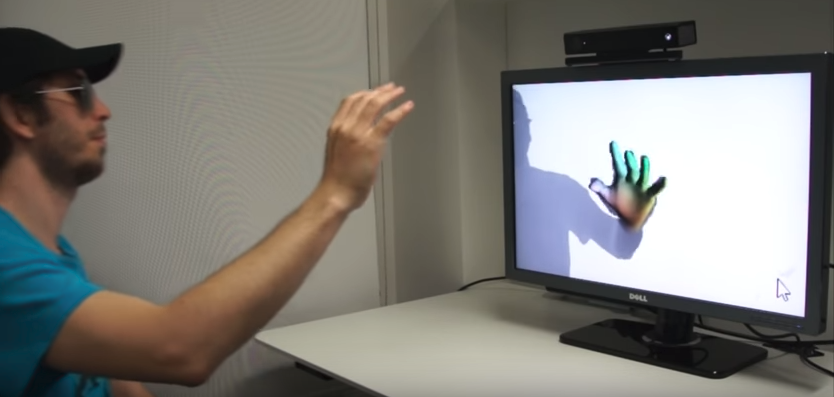
\includegraphics[width=0.85\linewidth]{hand_tracking}}
    \caption{Example of articulated hand tracking, reprinted from~\cite{taylor2016efficient}.}
    \label{fig:hand_tracking}
\end{figure}

\subsection{Data-driven body models}
Data-driven statistical body models built from large database of human 3D scans are receiving increasing attention from the research community. Having been trained on examples of real humans of a range of different shapes and adopting various poses, these models capture subtle details that is hard to encode explicitly. In part due to a good choice of training candidates, SCAPE~\cite{anguelov05scape}, FAUST~\cite{bogo2014faust} and SMPL~\cite{loper15smpl} models exemplify this technique and are able to account for many body shapes, poses and non-rigid deformations such as muscle bulging due to joint articulation. The quality of such models is such that a user can construct visually-realistic bodies that were never present in the original data. A noteable drawback of such approaches is the required time and financial investment in conducting the data capture and the subsequent need to align each scan.

SMPL first learns how human beings deform through pose changes using 1786 high-resolution 3D scans of different subjects in a wide variety of poses. Following alignment to a template mesh, a linear model for each biological gender is created from the CAESAR dataset \cite{robinette2002civilian} using principal component analysis (PCA). SMPL was motivated by the ambition to generate a realistic data-driven human body model which can be rendered in real-time using standard engines, such as Unity~\cite{unity2017} or Blender~\cite{blender2017}. Having been designed for animation, SMPLs base template has a number of useful qualities for this work; the underlying mesh is a clean structure and comprises relatively few polygons. A novelty of this model is that it encodes explicit and meaningful body joint positions. Some sample SMPL meshes are shown in Figure \ref{fig:smpl_model}.

\begin{figure}[H] % Example image
    \center{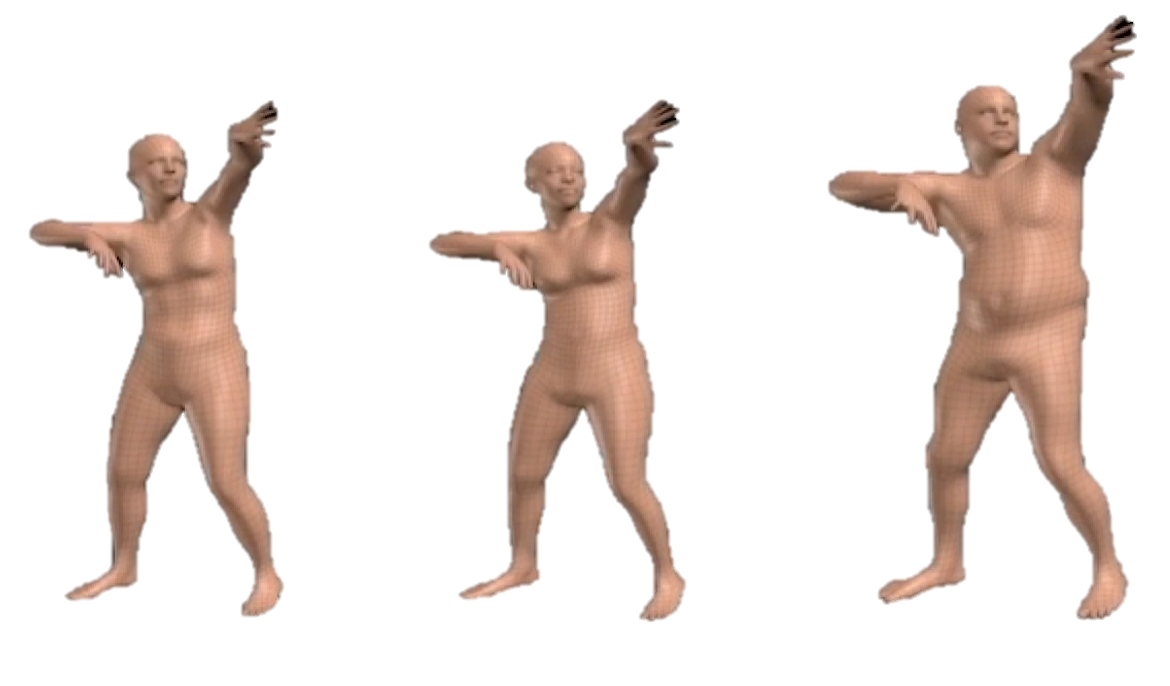
\includegraphics[width=0.5\linewidth]{smpl_wbg}}
    \caption{SMPL model showing pose-invariant shape changes, reprinted from~\cite{loper15smpl}.}
    \label{fig:smpl_model}
\end{figure}

A similar technique to that used to build the SMPL model has been recently used to build a Skinned Multi-Animal Linear Model (SMAL)~\cite{zuffi2017menagerie}, a generative animal model exhibiting realistic 3D shape (see Figure \ref{fig:smal_model_shape}) and pose (see Figure \ref{fig:smal_model_poses}). Due to the lack of available motion capture data for animal subjects, the SMAL model is learnt from a set of $41$ 3D scans of toy figurines in arbitrary poses. The figurines span five quadruped families, and included examples of lions, cats, tigers, dogs, horses, any many more, although notably for this work no rodent toys were included. The paper introduces a new technique to accurately align each toy scan to a common template, allowing the shape space to be learnt.

\begin{figure}[H]
    \centering
    \begin{subfigure}{0.3\linewidth}
    \centering
        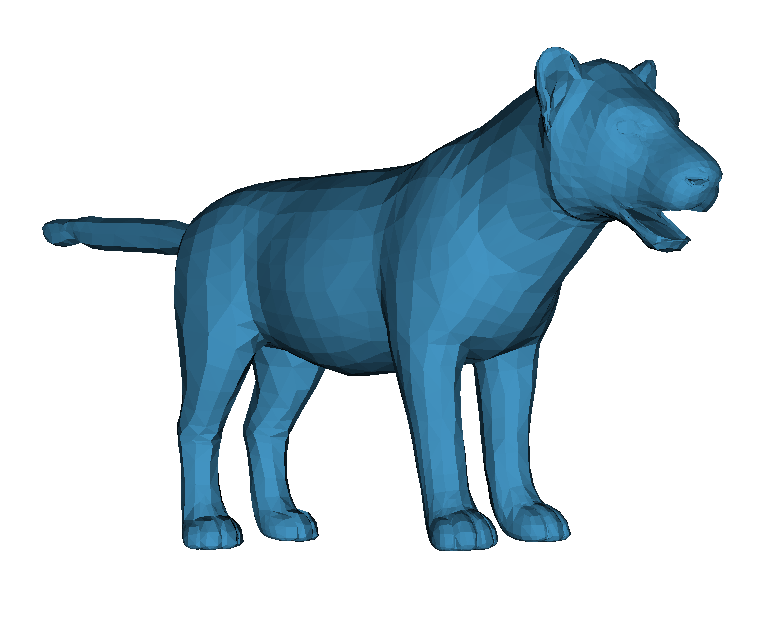
\includegraphics[width=1\linewidth]{smal/default}
        \caption{Default SMAL mesh.}
    \end{subfigure}%
    \begin{subfigure}{0.3\linewidth}
    \centering
        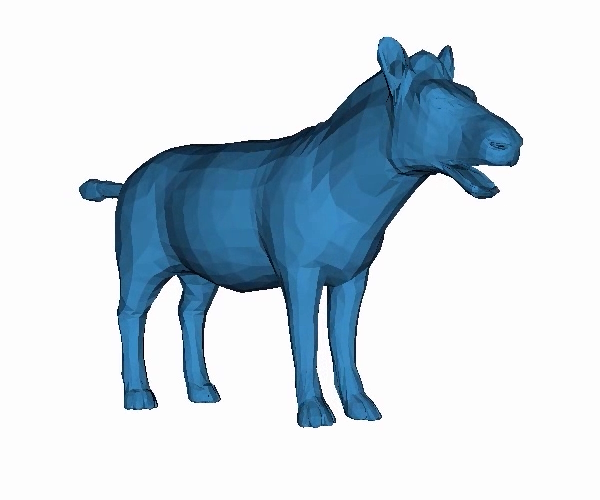
\includegraphics[width=1\linewidth]{smal/horse}
        \caption{SMAL in horse shape.}
    \end{subfigure}%
    \begin{subfigure}{0.3\linewidth}
        \centering
            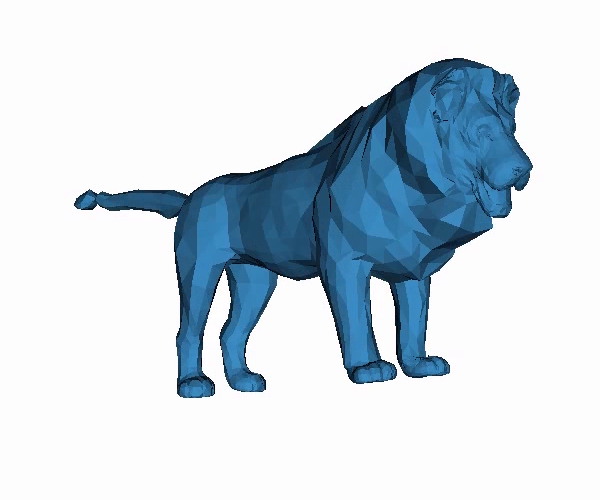
\includegraphics[width=1\linewidth]{smal/lion}
            \caption{SMAL in lion shape.}
    \end{subfigure}%
    \caption{SMAL with varying shape parameters.}
    \label{fig:smal_model_shape}
    \end{figure}

    \begin{figure}[H]
    \centering
    \begin{subfigure}{0.3\linewidth}
    \centering
        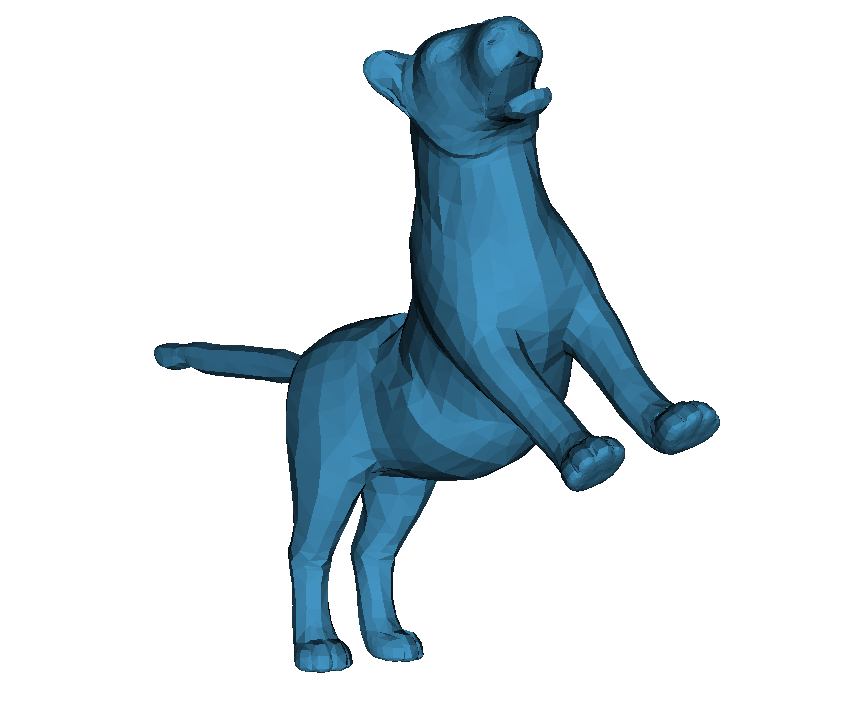
\includegraphics[width=1\linewidth]{smal/pose_1}
    \end{subfigure}%
    \begin{subfigure}{0.3\linewidth}
    \centering
        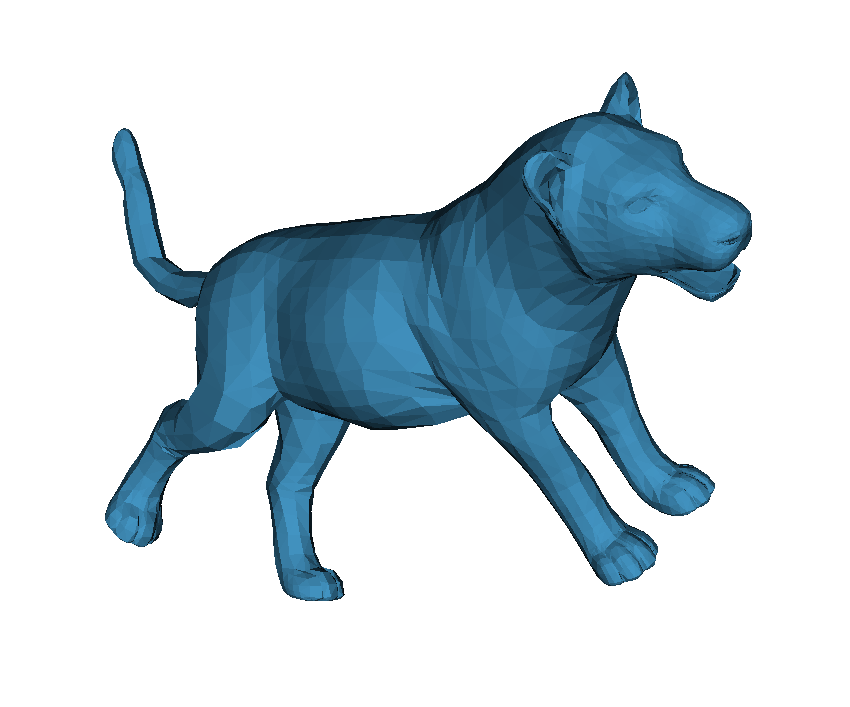
\includegraphics[width=1\linewidth]{smal/pose_2}
    \end{subfigure}%
    \begin{subfigure}{0.3\linewidth}
        \centering
            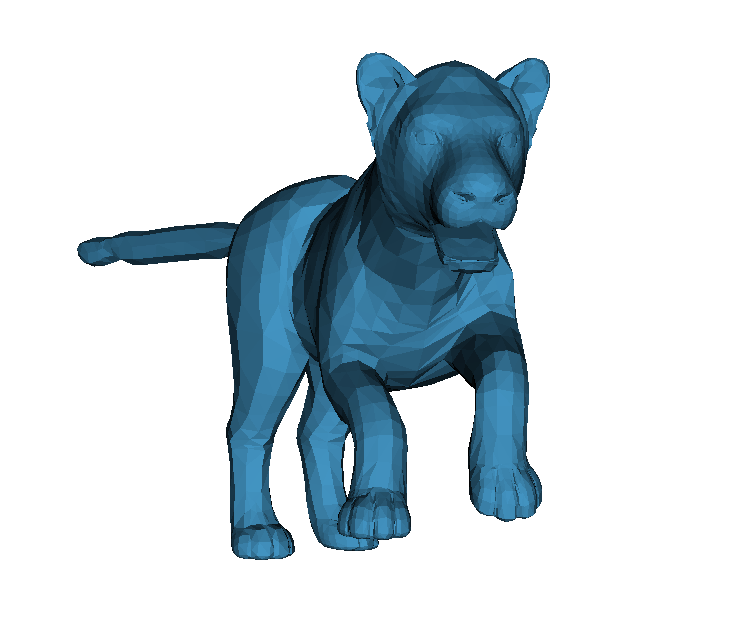
\includegraphics[width=1\linewidth]{smal/pose_3}
    \end{subfigure}%
    \caption{SMAL with varying pose parameters.}
    \label{fig:smal_model_poses}
\end{figure}

From the paper, SMAL is defined as a function $M(\beta, \theta, \gamma)$ parameterized by pose-invariant shape $\beta$, pose $\theta$ (including global rotation) and global translation $\gamma$. The function returns a triangulated surface comprising $6890$ vertices. SMAL contains $41$ shape parameters $\beta$ which are coefficients of a low-dimensional shape space. There are three pose parameters for each of the $32$ body joints and an additional three to express the global rotation. Global translation $\gamma$ is expressed by a further three parameters.

\subsubsection{Fitting the SMPL mesh to human images}
SMPLify \cite{bogo16keep} is a fully-automated optimization approach that uses predicted human joint positions to constrain a optimizer that fits the aforementioned SMPL model to RGB input images. It first makes use of the DeepCut CNN to predict 2D human body joints $J_{\text{est}}$ on input frames. For each 2D joint $i$ the CNN is able to provide a confidence value $w_i$ for the joint's position. The optimization begins by first solving for global rotation (i.e. $\theta_{0..2}$) and global translation $\gamma$ by fitting a small number of 2D torso points $J_{\text{torso}} \subset J_{\text{est}}$ to the data. The user is expected to provide a value for the focal length $f$. Then, the full optimization takes place, fitting 3D pose and shape to all 2D joints by minimizing the following objective function which comprises five error terms:

\begin{equation}
E(\beta, \theta) = E_{J}(\beta, \theta; K, J_{\text{est}}) + \lambda_{\theta}E_{\theta}(\theta) + \lambda_{\alpha}E_{\alpha}(\theta) + \lambda_{\text{sp}}E_{\text{sp}}(\theta; \beta) + \lambda_{\beta}E_{\beta}(\beta)
\end{equation}
where $\lambda$ terms are the scalar weights. The term $E_{J}$ is often referred to as the \textit{data} term, as it places most emphasis on constraining the model to the input sensory data. The job of this term is to penalize the weighted 2D distance between estimated joints $J_{\text{est}}$ and corresponding projected SMPL joints. In practice, this projection takes place using the OpenDR differentiable rendering framework to ensure the final formulation remains differentiable:

\begin{equation}
    E_{J}(\beta, \theta; K, J_{\text{est}}) = \sum_{joint j} w_{j} \rho(\Pi_{K}(R_{\theta}(J(\beta)_j)) - J_{\text{est}, j})
\end{equation}
where $J(\beta)$ is a function which predicts 3D body joints from body shape and $R_{\theta}(J(\beta))$ therefore denote posed 3D joints.

The remaining terms are now briefly discussed:
\clearpage
\begin{itemize}
    \item $E_{\theta}(\theta)$ is referred to as a \textit{pose prior} which favours more likely poses by assigning large punishment to those that deviate from known poses collected from a large dataset.
    \item $E_{\beta}(\beta)$ is referred to as a \textit{shape prior} which favours more likely pose-invariant shape configurations by assigning large punishment to those that deviate from known shapes collected from a large dataset. 
    \item $E_{\alpha}(\theta)$ is a \textit{joint limit} prior which ensures particular joints remain within acceptable angle limits. For example, a knee joint in a human model should be prohibited from bending more than 5 degrees upwards.
    \item $E_{sp}(\theta; \beta)$ is an \textit{interpenetration} term, which can only be defined in such shape modelling approaches. Using both shape and pose from the model, it is possible to determine if any limbs are self-intersecting, or intersect other parts of the body and assign appropriate penalty.
\end{itemize}

An example result can be seen in Figure \ref{fig:smplify}:

\begin{figure}[H] % Example image
    \center{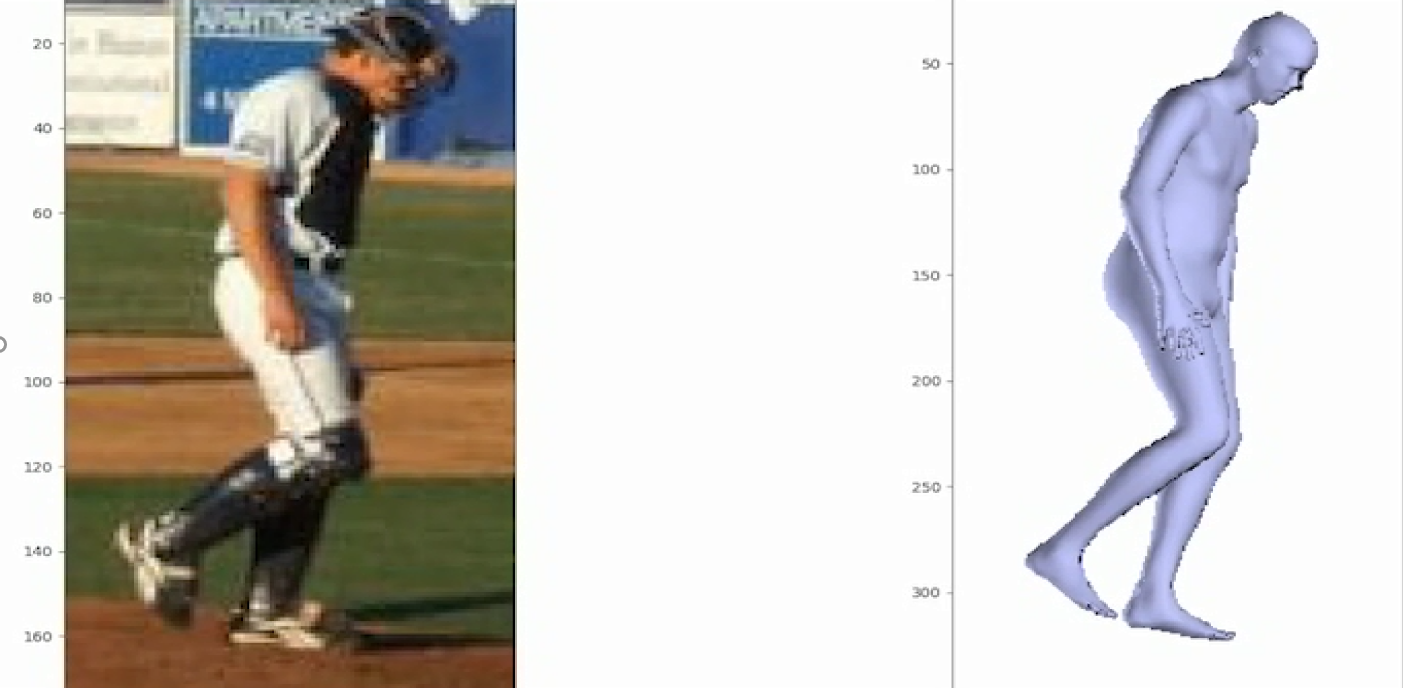
\includegraphics[width=0.95\linewidth]{fitting_smpl}}
    \caption{SMPLify: Fitting the SMPL model to the Leeds Sports Dataset.}
    \label{fig:smplify}
\end{figure}

\subsubsection{Fitting the SMAL mesh to animal images}
The SMAL paper briefly discusses a modification to the SMPLify approach in order to fit the SMAL model to RGB animal input images. The terms are largely the same, although the interpenetration term is omitted and joint positions are provided manually, rather than being predicted by a CNN. Finally, the optimizer requires a pre-segmented (i.e.\ silhouette) image which is also supplied by a user. An approach discussed in Chapter 4 builds on this work, so an in-depth description of this method is ommited here. However, an example result showing the result of the optimizer fitting the SMAL mesh to an RGB image of a fox can be seen in Figure \ref{fig:smalify}. Note that the whole optimization process takes around 1 minute per frame.

\begin{figure}[H] % Example image
    \center{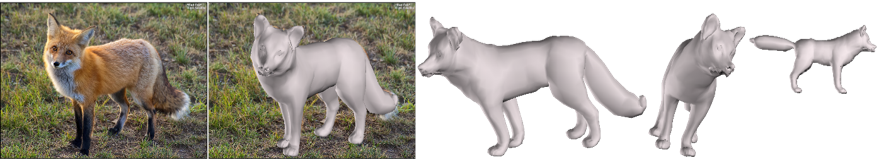
\includegraphics[width=0.95\linewidth]{fitting_smal}}
    \caption{Fitting SMAL to a hand segmented animal, reprinted from~\cite{zuffi2017menagerie}.}
    \label{fig:smalify}
\end{figure}

        
\subsection{Direct regression}
The most recent, and state-of-the-art approaches employ deep learning techniques to solve the entire optimization problem by directly regressing to shape and pose parameters of the template model. Tekin et al.~\cite{tekin2016direct} introduce a convolutional network trained on the Human3.6m dataset~\cite{lin2014microsoft} that directly regresses to a human pose defined in terms 3D locations $y \in \mathbb{R}^{3J}$ of $J$ body joints relative to a root joint. Tan et al.~\cite{tan17indirect} introduce an approach that directly regresses to SMPL parameters from synthetic images, ensuring suitable image jitters are applied to promote generality to real-world images. The method is termed Indirect Learning, and is trained from real human images with no known corresponding SMPL parameters. An autoencoder network is introduced, and a decoder first trained from synthetic (SMPL parameter, rendered image) pairs to construct an automatic renderer. This part of the network is then frozen, before the entire autoencoder is trained on many segmented human images that optimize the encoder to real-world examples. The end result is a process that is able to predict SMPL parameters from real-world human images. An example result is shown in Figure~\ref{fig:indirect_learning}.

\begin{figure}[H] % Example image
    \center{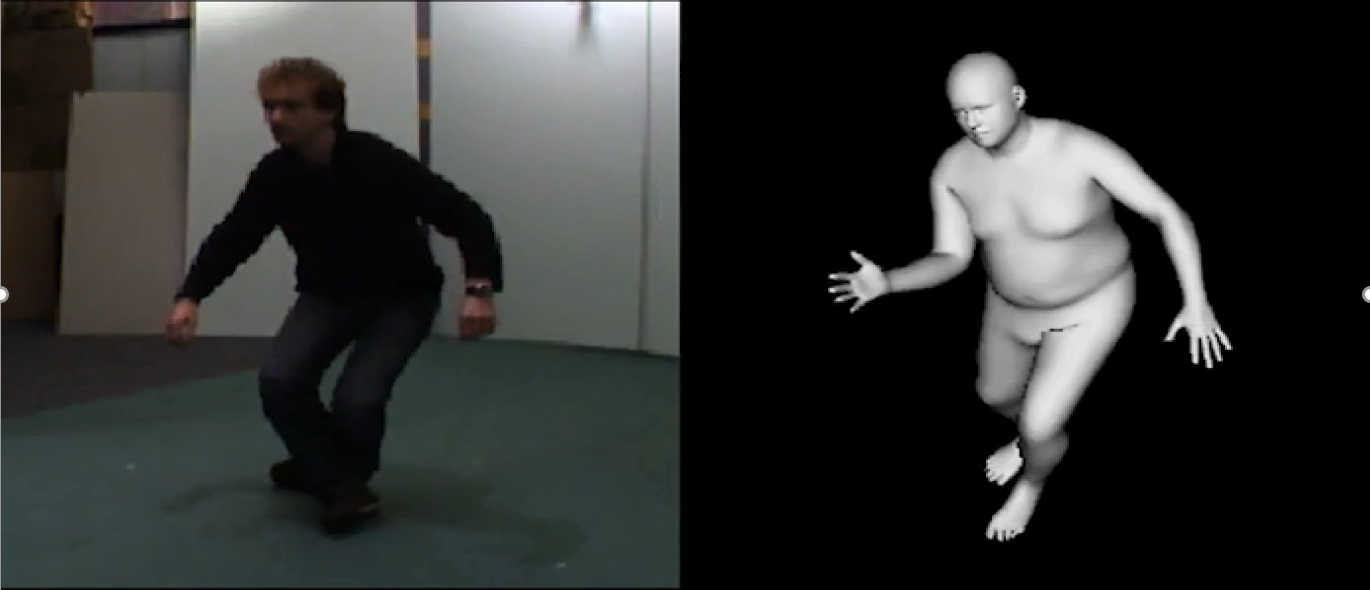
\includegraphics[width=0.75\linewidth]{indirect_learning}}
    \caption{Indirect learning method regressing to SMPL parameters from an RGB video sequence. Reprinted from~\cite{tan17indirect}.}
    \label{fig:indirect_learning}
\end{figure}


    
% \section{Obtaining animal test data}
%     A significant drawback due to the lack of available training data is that state-of-the-art segmentation pipelines require a wealth of (RGB Input, Segmentation) and (IR Input, Segmentation training pairs which are not readily available for animal targets. To resolve this, a collaborative project is underway between GSK and Texuna to design a bespoke camera module which can be fit into rodent, dog, mini-pig and rabbit enclosures. Figure \ref{fig:texuna_cage} shows a recent prototype design. The cameras are able to flip between RGB and IR capture modes and use IP camera technology, which is supported by a number of off-the-shelf recording systems. Once animal data is successfully recorded, it will be passed to human annotators to create a suitable dataset to train a segmentation network. Until this has been obtained, the system is designed on the premise of receiving perfect silhouette segmentations. 

%     % Talk a little more about the data -- problems (all outside?), occlusions, pets, number of pictures per animal (distribution) 
%     For testing, there are examples of real-world animal segmentations that form a satisfactory set for system testing. Between the Weizmann Horse Dataset~\cite{weizmann}, the IIIT-OXFORD PET dataset~\cite{oxfordpetdata} and animal superclasses from popular datasets such as MS Coco~\cite{lin2014microsoft} and PASCAL VOC~\cite{everingham2010pascal}, there are approximately one thousand RGB-segmentation pairs for independent images (i.e.\ not part of an available video sequence). It is worth noting that the distribution of images is heavily weighted towards cats, dogs and horses over other animal species. Moreover, images tend to be taken in outdoor environments with side-on animal views. This bias has been partially resolved by sourcing an additional 1500 frames from YouTube and the BBC Blue Planet II documentary series\footnote{Appropriate permissions have been sought where applicable}. These sequences were all segmented by hand, using the RotoBrush tool provided by the Adobe After-Effects~\cite{Bai:2009:VSC} package.  


\newcommand{\awfhang}[1]{
\begin{minipage}[t]{\textwidth}% Top-hanging minipage, will align on
                               % bottom of first line
\begin{tabbing} % tabbing so that minipage shrinks to fit
\\[-\baselineskip] % Make first line zero-height
#1 % Include user's text
\end{tabbing}
\end{minipage}} % can't allow } onto next line, as {WIDEBOX}~x will not tie.

\newcolumntype{L}[1]{>{\RaggedRight\hspace{0pt}}p{#1}}
\newcolumntype{R}[1]{>{\RaggedLeft\hspace{0pt}}p{#1}}

\begin{table}[t!]
{\sffamily
\scriptsize
\def\hd#1{\awfhang{#1}}
\begin{tabular}{@{}L{20mm}%Paper
|L{12mm}%Class
L{15mm}%Train
|L{15mm}%Template
L{17mm}%Video
L{17mm}%Test
|L{9mm}%Model
L{5mm}%Size
@{}}
\hd{Paper}%
&\hd{Animal\\Class}%
&\hd{Training\\requirements}%
&\hd{Template\\Model}%
&\hd{Video\\required}%
&\hd{Test Time\\Annotation}%
&\hd{Model\\Fitting}%
&\hd{Test\\Size}%
\\\hline
%%%%%%%%%%%%%%%%%%%%%%
This paper
& Dogs  % 2D Joints, Silhouettes, 3D Template, 3D Priors
& J2, S2, T3, P3
& SMAL
& No & None & No & 1703
\\\hline
%%%%%%%%%%%%%%%%%%%%%%
3D-Safari~\cite{Zuffi19Safari}        
& Zebras, horses
% 3D models (albeit synthetic), 2D Joints,  Silhouettes,  3D Priors
& M3 (albeit synthetic), J2, S2, P3
& SMAL
& 3-7 frames / animal & None & Yes & 200
\\\hline
%%%%%%%%%%%%%%%%%%%%%%
Lions, Tigers and Bears (SMALR)~\cite{zuffi_lions} 
& MLQ
& Not trained
& SMAL
& 3-7 frames / animal & J2, S2 & Yes & 14
\\\hline
%%%%%%%%%%%%%%%%%%%%%%
3D Menagerie (SMAL)~\cite{zuffi2017menagerie}                
& MLQ 
& Not trained
& SMAL
& No & J2, S2 & Yes & 48 
\\\hline
%%%%%%%%%%%%%%%%%%%%%%
Creatures Great and SMAL~\cite{biggs2018creatures}
& MLQ
& Not trained
& SMAL
& Yes & S2 (for best results shown) & Yes & 9             \\\hline 
%%%%%%%%%%%%%%%%%%%%%%
Category Specific Mesh Reconstructions~\cite{kanazawa2018birds}
& Birds
& J2, S2
& Bird convex hull
& No & None & No & 2850          
\\\hline
%%%%%%%%%%%%%%%%%%%%%%
What Shape are Dolphins~\cite{cashman2013shape}
& Dolphins, Pigeons 
& Not trained
& Dolphin Template
& 25 frames / category & J2, S2 & Yes & 25
\\\hline
%%%%%%%%%%%%%%%%%%%%%%
Animated 3D Creatures~\cite{reinert2016animatedsketching}
& MLQ
& Not trained
& Generalized Cylinders
& Yes & J2, S2 & Yes & 15
\\\hline
\end{tabular}
}
\caption{Literature summary: Our paper extends large-scale ``in-the-wild'' reconstruction to the difficult class of diverse breeds of dogs. 
MLQ: Medium-to-large quadrupeds. J2: 2D Joints. S2: 2D Silhouettes. T3: 3D Template. P3: 3D Priors. M3: 3D Model.}
\label{tab:literature}
% \vspace{-8mm}
\end{table}

\section{CGAS Paper}
3D animal tracking is relatively new to the computer vision literature, but animal breed identification is a well studied problem~\cite{imagenet_cvpr09}. Video tracking benchmarks often use animal sequences~\cite{DAVIS2017-1st,DAVIS2017-2nd}, although the tracking output is typically limited to 2D affine transformations rather than the detailed 3D mesh that we propose.  Although we believe our work is the first to demonstrate dense 3D tracking of animals in video without the need for user-provided keypoints, we do build on related work across computer vision:

\subsubsection*{Morphable shape models.}
Cashman and Fitzgibbon~\cite{cashman2013shape} obtained one of the first 3D morphable animal models, but their work was limited to small classes of objects (e.g. dolphins, pigeons), and did not incorporate a skeleton.  Their work also showed the use of the 2D silhouette for fitting, which is key to our method. 
Reinert {\em et al.} \cite{reinert2016animated} meanwhile construct 3D meshes by fitting generalized cylinders to hand-drawn skeletons.
Combined skeletal and morphable models were used by Khamis {\em et al.}~\cite{hand-shape} for modelling the human hand, and Loper {\em et al.}~\cite{loper15smpl} in the SMPL model which has been extensively used for human tracking. 

The SMPL model was extended to animals by Zuffi {\em et al.}~\cite{zuffi2017menagerie}, where the lack of motion capture data for animal subjects is cleverly overcome by building the model from $41$ 3D scans of toy figurines from five quadruped families in arbitrary poses. Their paper demonstrates single-frame fits of their model to real-world animal data, showing that despite the model being built from ``artists' impressions'' it remains an accurate model of real animals. This is borne out further by our work.  Their paper did however depend on per-frame human annotated keypoint labels, which would be costly and challenging to obtain for large video sequences. This work was recently extended~\cite{zuffi_lions} with a refinement step that optimizes over model vertex positions. This can be considered independent to the initial SMAL model fit and would be trivial to add to our method.

\subsubsection*{Shape from silhouette.} Silhouette images have been shown to contain sufficient shape information to enable their use in many 3D recovery pipelines. Chen {\em et al.}~\cite{chen2010inferring} demonstrate single-view shape reconstruction from such input for general object classes, by building a shape space model from 3D samples. More related to our work, Favreau {\em et al.}~\cite{favreau2004animal} apply PCA to silhouette images to extract animal gaits from video sequences. The task of predicting silhouette images from 2D input has been effectively used as a proxy for regressing 3D model parameters for humans~\cite{tan17indirect,kanazawa18end-to-end} and other 3D objects~\cite{wiles2017silnet}.

\subsubsection*{Joint position prediction.} There is an extensive body of prior work related to joint position prediction for human subjects. Earlier work used graphical approaches such as pictorial structure models~\cite{andriluka2010monocular,pishchulin2013poselet,johnson2010clustered}, which have since been replaced with deep learning-based methods~\cite{cao2017realtime,bulat2016human}. Few works predict animal joint positions directly owing to the lack of annotated data, although Mathis {\em et al.}~\cite{mathis2018deeplabcut} demonstrate the effectiveness of human pose estimation architectures for restricted animal domains. Our method instead trains on silhouette input, allowing the use of synthetic training imagery. The related task of animal part segmentation~\cite{wang2015joint,wang2015semantic} has seen some progress due to general object part datasets~\cite{chen_cvpr14,zhou2017scene}.




The closest work in terms of scale is the category-specific mesh reconstruction of Kanazawa et al.~\cite{kanazawa2018birds}, where 2850 images of birds were reconstructed.  However doing so for the complex pose and shape variations of dogs required the advances described in this paper.

Table~\ref{tab:literature} summarizes previous work on animal reconstruction.
It is interesting to note that while several papers demonstrate reconstruction across species, which {\em prima facie} is a richer class than just dogs, the test-time requirements (e.g. manually-clicked keypoints/silhouette segmentations, input image quality etc.) are considerably higher for those systems.
Thus we claim that the achievement of reconstructing a full range of dog breeds, 
with variable fur length, varying shape and pose of ears, and with considerable occlusion, is a significant contribution.

\section{Dog Paper}

% \textbf{Monocular 3D reconstruction of human bodies}
\subsubsection{Monocular 3D reconstruction of human bodies}
The majority of recent work in 3D pose and shape recovery from monocular images tackles the special case of 3D \emph{human} reconstruction. As a result, the research community has collected a multitude of open source human datasets which provide strong supervisory signals for training deep neural networks. These include accurate 3D deformable template models~\cite{loper15smpl} generated from real human scans, 3D motion capture datasets~\cite{ionescu2013human3,vonmarcard2018recovering} and large 2D datasets~\cite{lin2014microsoft,johnson2010clustered,andriluka14cvpr} which provide keypoint and silhouette annotations. 

The abundance of available human data has supported the development of successful monocular 3D reconstruction pipelines~\cite{kolotouros19convolutional,kanazawa18end-to-end}. Such approaches rely on accurate 3D data to build detailed priors over the distribution of human shapes and poses, and use large 2D keypoints datasets to promote generalization to ``in-the-wild'' scenarios. Silhouette data has also been shown to assist in accurate reconstruction of clothes, hair and other appearance detail~\cite{pifuSHNMKL19,alldieck2019learning}.
While the dominant paradigm in human reconstruction is now end-to-end deep learning methods, SPIN~\cite{kolotouros19learning} show impressive improvement by incorporating an energy minimization process within their training loop to further minimize a 2D reprojection loss subject to fixed pose \& shape priors. Inspired by this innovation, we learn an iteratively-improving shape prior by applying expectation maximization during the training process.

\textbf{Monocular 3D reconstruction of animal categories.}
While animals are often featured in computer vision literature, there are still relatively few works that focus on accurate 3D animal reconstruction. 

A primary reason for this is absence of large scale 3D datasets\footnote{Released after the submission of this paper, RGBD-Dog dataset~\cite{Kearney_2020_CVPR} is the first open-source 3D motion capture dataset for dogs.} stemming from the practical challenges associated with 3D motion capture, as well as a lack of 2D data which captures a wide variety of animals. The recent Animal Pose dataset~\cite{animalpose} is one such 2D alternative, but contains significantly fewer labelled images than our new StanfordDogs dataset (4,000 compared to 20,580 in ). 
On the other hand, animal silhouette data is plentiful~\cite{lin2014microsoft,everingham2010pascal,DAVIS2017-2nd}.

%In part due to the practical challenges associated with motion capture of animal categories, there is a severe lack of 3D animal data which could be used to build accurate 3D deformable models or supervise 3D predictions~\footnote{Released after the submission of this paper, RGBD-Dog dataset~\cite{Kearney_2020_CVPR} is the first open-source 3D motion capture dataset for dogs.}. 

Zuffi et al.~\cite{zuffi2017menagerie} made a significant contribution to 3D animal reconstruction research by releasing SMAL, a deformable 3D quadruped model (analagous to SMPL~\cite{loper15smpl} for human reconstruction) from $41$ scans of artist-designed toy figurines. The authors also released shape and pose priors generated from artist data. In this work we develop \emph{SMBLD}, an extension of SMAL that better represents the diverse dog category by adding scale parameters and refining the shape prior using our large image dataset.

While there have been various ``model-free'' approaches which do not rely on an initial template model to generate the 3D animal reconstruction, these techniques often do not produce a mesh~\cite{Agudo_2018_CVPR,novotny19c3dpo} or rely heavily on input 2D keypoints or video at test-time~\cite{vicente_3dv,Probst2018_ECCVa}. An exception is the end-to-end network of Kanazawa et al.~\cite{kanazawa2018birds}, although we argue that the bird category exhibits more limited articulation than our dog category.

We instead focus on model-based approaches. The SMAL authors~\cite{zuffi2017menagerie} demonstrate fitting their deformable 3D model to quadruped species using user-provided keypoint and silhouette dataset. SMALR~\cite{zuffi_lions} then demonstrated fitting to broader animal categories by incorporating multi-view constraints from video sequences. Biggs et al.~\cite{biggs2018creatures} overcame the need for hand-clicked keypoints by training a joint predictor on synthetic data. 3D-Safari~\cite{Zuffi19Safari} further improve by training a deep network on synthetic data (built using SMALR~\cite{zuffi_lions}) to recover detailed zebra shapes in the wild.

A drawback of these approaches is their reliance on a test-time energy-based optimization procedure, which is susceptible to failure with poor quality keypoint/silhouette predictions and increases the computational burden. By contrast our method requires no additional energy-based refinement, and is trained purely from single in-the-wild images. The experimental section of this paper contains a robust comparison between our end-to-end method and relevant optimization-based approaches. 


A major impediment to research in 3D animal reconstruction has been the lack of a strong evaluation benchmark, with most of the above methods showing only qualitative evaluations or providing quantitative results on fewer than 50 examples. To remedy this, we introduce \emph{StanfordExtra}, a new large-scale dataset which we hope will drive further progress in the field. 
